%% LUMEN manuscript, MDPI Remote Sensing LaTeX class. Generated by paper/build_latex.py from
%% paper/MANUSCRIPT.md: edit paper/manuscript_src/*.md and rebuild rather than editing this file.
\documentclass[remotesensing,article,submit,pdftex,moreauthors]{Definitions/mdpi}

\firstpage{1}
\makeatletter
\setcounter{page}{\@firstpage}
\makeatother
\pubvolume{1}
\issuenum{1}
\articlenumber{0}
\pubyear{2026}
\copyrightyear{2026}
\datereceived{ }
\daterevised{ }
\dateaccepted{ }
\datepublished{ }
\hreflink{https://doi.org/}

%% ---- working draft: no journal boilerplate (MDPI's class file is left unchanged) ----
\makeatletter
\renewcommand{\contentleftcolumn}{}                           % left column: editor, dates, copyright
\let\LUMEN@includegraphics\includegraphics                    % MDPI and journal logos
\renewcommand{\includegraphics}[2][]{\IfSubStr{#2}{Definitions/logo}{}{\LUMEN@includegraphics[#1]{#2}}}
\fancypagestyle{plain}{\fancyhf{}\renewcommand{\headrulewidth}{0pt}\renewcommand{\footrulewidth}{0pt}}
\fancyhf{}
\rhead{\fontsize{8}{8}\selectfont\thepage{} of \pageref*{LastPage}}
\renewcommand{\headrulewidth}{0pt}
\renewcommand{\footrulewidth}{0pt}
\makeatother

\addhighlights{yes}
\renewcommand{\addhighlights}{%
\noindent\textbf{What are the main findings?}
\begin{itemize}[labelsep=2.5mm,topsep=-3pt]
\item A one-dimensional network pretrained on 400,000 Hapke-simulated lunar soils and fine-tuned on 19 returned soils predicts FeO, four other oxides, seven-part mineralogy and maturity. On identical laboratory data it cuts FeO error by 42\% relative to a published wavelet--autoencoder pipeline and is significantly more accurate than a tuned random forest on 8 of 13 targets.
\item Conformal intervals reach nominal coverage, and an identifiability gate withholds olivine and minor glasses, which no tested method predicts better than a zero-information baseline.
\end{itemize}\vspace{3pt}
\noindent\textbf{What are the implications of the main findings?}
\begin{itemize}[labelsep=2.5mm,topsep=-3pt]
\item Most of the error of physics-only inversions is removed by calibrating against returned soils, not by added model complexity.
\item Laboratory skill does not transfer to orbit: at 49 returned-sample sites, orbitally fine-tuned LUMEN (3.27 wt\% FeO) does not significantly improve on the published pipeline (3.58 wt\%) and is outperformed by a two-band linear regression (2.11 wt\%).
\end{itemize}
}

\Title{Physics-Pretrained, Sample-Calibrated Deep Learning for Lunar Soil FeO, Mineralogy and Maturity from Moon Mineralogy Mapper Spectra}
\TitleCitation{Physics-Pretrained, Sample-Calibrated Deep Learning for Lunar Soil FeO, Mineralogy and Maturity from Moon Mineralogy Mapper Spectra}
\Author{}
\AuthorNames{}
\isAPAStyle{\AuthorCitation{}}{\isChicagoStyle{\AuthorCitation{}}{\AuthorCitation{}}}
\address{}
\corres{}

\abstract{Lunar soil composition is retrieved from reflectance spectra by empirical regressions, radiative-transfer inversions and physics-guided networks, which are rarely compared on identical data or given calibrated uncertainties. We present LUMEN, a one-dimensional convolutional network pretrained on 400,000 soils from a domain-randomised Hapke simulator with nanophase-iron space weathering, fine-tuned on laboratory spectra of the 19 Lunar Soil Characterization Consortium soils, with conformal prediction intervals and an identifiability gate that withholds outputs without demonstrable skill. Under leave-one-soil-out evaluation with a protocol fixed before scoring, LUMEN predicts FeO to 1.26 wt\% and TiO$_{2}$ to 0.70 wt\%, reduces the FeO error of a published wavelet--autoencoder pipeline by 42\% and the mineral-proportion errors of a Shkuratov-model inversion by 54--74\%, and, with its configuration chosen inside the cross-validation, is significantly more accurate than a tuned random forest on 8 of 13 targets. Intervals reach nominal coverage; olivine is not identifiable. On Moon Mineralogy Mapper spectra at 49 returned-sample sites, the laboratory model does not transfer (6.81 wt\%); after orbital fine-tuning it reaches 3.27 wt\% under leave-one-landing-site-out, not significantly better than the published pipeline (3.58 wt\%) and significantly worse than a two-band linear regression (2.11 wt\%).}
\keyword{lunar regolith; FeO; mineral abundance; space weathering; Moon Mineralogy Mapper; Hapke model; deep learning; transfer learning; conformal prediction; uncertainty quantification}

\begin{document}

\section{Introduction}

The iron and titanium content, modal mineralogy and space-weathering maturity of the lunar regolith record the Moon's crustal and volcanic history and constrain the use of its resources. The Moon Mineralogy Mapper (M$^{3}$) on Chandrayaan-1 acquired visible to near-infrared reflectance spectra over most of the surface~\cite{pieters2009,green2011}. These spectra carry the crystal-field absorptions of Fe$^{2+}$ in pyroxene and olivine near 1 and 2 $\upmu$m, overprinted by the darkening and reddening of nanophase metallic iron, and turning them into quantitative composition remains an inverse problem with little ground truth.

Empirical methods relate spectral parameters to the composition of returned samples at their landing sites. The Clementine band-ratio algorithms of Lucey et al.~\cite{lucey2000} remain the reference for FeO and TiO$_{2}$, and band parameters of the 1 and 2 $\upmu$m absorptions have been calibrated for M$^{3}$~\cite{bhatt2012,bhatt2015}. Regressions range from partial least squares~\cite{sun2016}, neural networks~\cite{xia2019} and support vector machines~\cite{wang2021} to systematic comparisons of regressors~\cite{qiu2022}, and convolutional networks on Kaguya Multiband Imager spectra produced global oxide maps once Chang'e-5~\cite{yang2023,zhang2023} and Chang'e-6~\cite{shi2026} samples were added; Diviner data~\cite{ma2022}, gradient boosting~\cite{wu2024} and random forests~\cite{fernandez2025} have also been used. The method this study builds on, by Fernández-Díaz et al.~\cite{fernandez2026}, combines a db4 wavelet decomposition, a deep autoencoder and a random-forest regressor into a global M$^{3}$ FeO map at 150 m per pixel. All of these methods are trained on about 50 sampling sites and evaluated on random splits or small hold-out sets, rarely on identical data alongside competing methods or against a zero-information baseline.

Physics-based methods model reflectance with radiative transfer. The Hapke model~\cite{hapke1993} and its treatment of nanophase iron~\cite{hapke2001,lucey2011,pieters2016} support inversions for mineral abundance, grain size and submicroscopic iron~\cite{lili2011,sunlucey2021,trang2019}; the Shkuratov model~\cite{shkuratov1999} has been inverted on M$^{3}$ by a network trained on synthetic spectra~\cite{korokhin2024}; Hapke inversions have been embedded in Bayesian samplers~\cite{jung2026}; and PGU-Net~\cite{lin2026} placed a Hapke single-scattering-albedo mixing layer inside a deep autoencoder for unsupervised unmixing, validated on M$^{3}$ only indirectly, against Kaguya products, with sample-informed priors named as the next step. Such inversions are interpretable but non-unique and sensitive to the end-member set and optical constants. Laboratory studies of the Lunar Soil Characterization Consortium (LSCC) soils have also combined spectra with measured mineralogy~\cite{li2012,grumpe2018,surkov2025}.

Our independent reproductions of three recent methods~\cite{fernandez2026,korokhin2024,jung2026} show where these approaches fall short. The network of Korokhin et al. recovers orthopyroxene, olivine and the grey absorber on its own synthetic test set with R$^{2}$ of only 0.06, 0.17 and 0.32, yet these quantities are mapped; in Jung et al., abundances drawn from the prior alone already meet two of the three published accuracy bounds; and in Fernández-Díaz et al., a random forest on the raw wavelet coefficients is more accurate than one on the autoencoder codes. Each point concerns how much of a retrieved number the spectrum determines and how that is tested, not the physical models themselves. What is missing is a method that uses physics as a source of training data, lets returned soils correct it, states its uncertainty and which outputs it cannot identify, and is evaluated against published pipelines on identical data, under grouped cross-validation and against a zero-information baseline.

We propose LUMEN (LUnar Mineralogy Estimation Network) to fill this gap. The main contributions are:

(1) \textbf{A hybrid physics--learning method.} A domain-randomised Hapke simulator, built from 49 lunar mineral and glass end-members (none taken from an evaluation soil) with physically modelled nanophase- and microphase-iron weathering, generates 400,000 synthetic soils. A compact one-dimensional convolutional network is pretrained on them and fine-tuned on returned soils, and from one spectrum predicts seven-part modal mineralogy, five oxides and maturity. A deep ensemble with conformal calibration supplies intervals with verified coverage, and an identifiability gate withholds every target whose skill over a zero-information baseline is not demonstrable.

(2) \textbf{An identical-data, protocol-fixed comparison.} LUMEN is compared with wavelet--autoencoder regression~\cite{fernandez2026}, Shkuratov-model inversion~\cite{korokhin2024}, Hapke--Bayesian inversion~\cite{jung2026} and classical regressors on the same 75 laboratory spectra and the same leave-one-soil-out and leave-one-mission-out folds, with paired tests corrected for multiple comparisons. Every evaluation choice was committed to version control before the first score was computed, and negative and null results are reported alongside positive ones.

(3) \textbf{A test of laboratory-to-orbit transfer.} Using M$^{3}$ spectra at the returned-sample sites on which the base method was calibrated~\cite{fernandez2026,qiu2025}, under both that method's own cross-validation and a spatially honest leave-one-landing-site-out protocol, we show that laboratory accuracy does not carry over to orbit without orbital labels, how much a small orbital fine-tuning set recovers, and that simple two-band regressions remain more accurate on orbit.

Section 2 describes the data, the physical preliminaries and the method; Section 3 reports the experiments; Section 4 discusses them, including limitations; and Section 5 concludes.

\section{Materials and Methods}

\subsection{Data and Preprocessing}

\subsubsection{Laboratory Spectra and Ground Truth}

We use the LSCC suite~\cite{taylor2001,taylor2010} of nine mare soils (Apollo 11, 12, 15 and 17) and ten highland soils (Apollo 14 and 16), each sieved into <10, 10--20, 20--45 and <45 $\upmu$m fractions and measured at the Reflectance Experiment Laboratory (RELAB)~\cite{relab2004} at 30$^{\circ}$ incidence and 0$^{\circ}$ emission; the 10--20 $\upmu$m spectrum of soil 70181 is absent, leaving 75 spectra. Point-count modal mineralogy (vol\%), available for the three finer fractions (56 spectra), is merged into seven parts: plagioclase (PLG), low-Ca pyroxene (LCP, orthopyroxene plus pigeonite), high-Ca pyroxene (HCP), olivine (OLV), ilmenite (ILM), agglutinitic glass (AGG) and other phases (OTH). Bulk FeO, TiO$_{2}$, Al$_{2}$O$_{3}$, CaO and MgO (wt\%) and the maturity index Is/FeO are available for all 75 spectra; the tables were checked against their own column sums and totals. Every spectrum is convolved to the 71 M$^{3}$ global-mode bands between 540.8 and 2497.1 nm with Gaussian responses whose width equals the band spacing, excluding the thermally affected channels beyond 2.5 $\upmu$m.

\subsubsection{End-Member Library}

The simulator draws on 49 RELAB spectra of lunar mineral separates and glasses (17 plagioclase, 7 low-Ca and 11 high-Ca pyroxene, 6 olivine, 4 ilmenite, 2 volcanic and 2 synthetic glasses) from mare basalts, highland rocks, one non-LSCC soil (62241) and synthetic glasses, each verified against its PDS4 metadata. An automatic check ensures that no end-member derives from any of the 19 evaluation soils; because every RELAB agglutinate separate comes from an LSCC soil, agglutinates are modelled physically instead (Section 2.3.1).

\subsubsection{M$^{3}$ Data}

All orbital data are M$^{3}$ Level-2 global-mode reflectance~\cite{green2011}. For mapping we use the Shapley-region strip M3G20090728T214215 analysed by Korokhin et al.~\cite{korokhin2024}, a block around the Apollo 16 landing site (M3G20090607T110414) and the two Aristarchus regions of interest of Jung et al.~\cite{jung2026}.

The FeO ground truth of the base method~\cite{fernandez2026} is the compilation of Qiu et al.~\cite{qiu2025jgr}, available in open access as Supplementary Table 1 of Qiu et al.~\cite{qiu2025}: 49 distinct, station-level sampling sites (Apollo 11--17 landing sites and traverse stations, Luna 16, 20 and 24, and Chang'e-3, -5 and -6) with laboratory FeO and Clementine reflectances at 415--1000 nm, which we verified against the worked example in~\cite{fernandez2026} (Apollo 17 LRV-12, 17.4 wt\% FeO). For each site, every M$^{3}$ strip whose nearest pixel lies within 0.01$^{\circ}$ of the site, at least five samples from the swath edge, contributes its 3 $\times$ 3-pixel block if at least 5 of the 9 pixels are valid (finite, 0 < R < 1 on M$^{3}$ bands 3--85, the band set of~\cite{fernandez2026}); the site spectrum is the per-band median over contributing strips. All 49 sites are covered, Chang'e-5 included, by 183 strips (one to six per site, median four). Every input file is listed in a SHA-256 manifest that each processing stage verifies at start and end.

\subsection{Preliminaries: Hapke Model, Single-Scattering Albedo and Space Weathering}

For an intimate particulate mixture we use the Hapke bidirectional reflectance~\cite{hapke1993},

\begin{equation}
r(w) = \frac{w}{4(\mu_0+\mu)}\,H(w,\mu_0)\,H(w,\mu)
\label{eq1}
\end{equation}

where $w$ is the single-scattering albedo (SSA) and $\mu_0$ and $\mu$ are the cosines of the incidence and emission angles (30$^{\circ}$ and 0$^{\circ}$ for RELAB). The phase function is isotropic and the opposition effect is neglected, which suits RELAB geometry, and $H$ is the approximate Chandrasekhar function

\begin{equation}
H(w,x) = \left[1 - w\,x\left(r_0 + \frac{1-2r_0x}{2}\ln\frac{1+x}{x}\right)\right]^{-1},\qquad r_0=\frac{1-\gamma}{1+\gamma},\ \gamma=\sqrt{1-w}
\label{eq2}
\end{equation}

Equation (1) is monotonic in $w$ and is inverted numerically from a dense table.

The SSA of a grain population with absorption coefficient $\alpha$, real index $n$, imaginary index $k$ and size $D$ follows the equivalent-slab model~\cite{hapke1993},

\begin{equation}
w = S_e + (1-S_e)\,\frac{(1-S_i)\,\Theta}{1-S_i\,\Theta},\qquad \Theta = e^{-\alpha\langle D\rangle}
\label{eq3}
\end{equation}

with

\begin{equation}
S_e = \frac{(n-1)^2+k^2}{(n+1)^2+k^2} + 0.05,\qquad S_i = 1.014 - \frac{4}{n(n+1)^2},\qquad \langle D\rangle = \frac{2}{3}\left[n^2-\frac{1}{n}(n^2-1)^{3/2}\right]D
\label{eq4}
\end{equation}

and $\alpha = 4\pi k/\lambda$ for a pure phase. For each end-member we invert Equations (1)--(4) at the separate's nominal grain size to obtain $k(\lambda)$. Because the reflectance is not monotonic in $k$, falling to an opacity floor and then rising as surface reflection grows, the root is bracketed on the physical, falling branch; every end-member then reproduces its own measured reflectance to < 10$^{-10}$.

Nanophase metallic iron (npFe$^{0}$) at volume fraction $\phi$ in a host of refractive index $n_h$ adds an absorption~\cite{hapke2001,lucey2011}

\begin{equation}
\alpha_{np}(\lambda) = \frac{36\pi\, z(\lambda)\,\phi}{\lambda},\qquad z = \frac{n_h^3\, n_{Fe}\, k_{Fe}}{\left(n_{Fe}^2-k_{Fe}^2+2n_h^2\right)^2+\left(2n_{Fe}k_{Fe}\right)^2}
\label{eq5}
\end{equation}

where $n_{Fe}$ and $k_{Fe}$ are the optical constants of iron. Microphase iron (mpFe$^{0}$) is a grey absorber, $\alpha_{mp} = 3\phi_{mp}/(4 r_{mp})$ with $r_{mp} = 0.1$ $\upmu$m, which darkens without reddening~\cite{lucey2011}. Components with volume fractions $f_i$, grain sizes $D_i$ and SSAs $w_i$ mix in SSA with cross-section weights,

\begin{equation}
w_{mix} = \frac{\sum_i (f_i/D_i)\,w_i}{\sum_i f_i/D_i}
\label{eq6}
\end{equation}

and the mixed SSA is converted to reflectance with Equation (1).

\subsection{Proposed Method: LUMEN}

LUMEN has four stages (Figure 1): a physics simulator generates labelled synthetic soils; a network is pretrained on them; it is fine-tuned on returned soils and, for orbital use, on M$^{3}$ spectra; and an uncertainty and identifiability layer decides what is reported.

\begin{figure}[H]
\begin{adjustwidth}{-\extralength}{0cm}
\centering
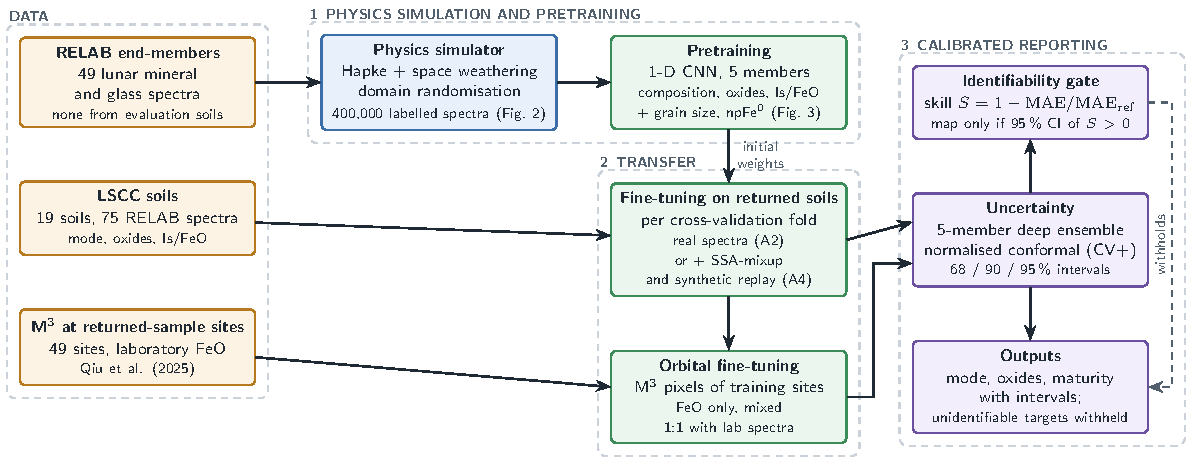
\includegraphics[width=\linewidth]{figures/fig_framework}
\end{adjustwidth}
\caption{Overview of LUMEN. Synthetic soils from the physics simulator (Figure 2) pretrain the network (Figure 3), which is then fine-tuned on laboratory spectra of returned soils and, optionally, on M$^{3}$ spectra at returned-sample sites. A five-member ensemble with conformal calibration provides prediction intervals, and the identifiability gate decides which targets are mapped.\label{fig1}}
\end{figure}

\subsubsection{Domain-Randomised Physics Simulator}

Each synthetic soil draws a petrological regime (feldspathic, basaltic or broad: Dirichlet priors on the crystalline proportions, truncated at $\leq$20\% ilmenite and $\leq$60\% olivine), a maturity that sets the agglutinate fraction, AGG = clip(0.65 $\cdot$ maturity + N(0, 0.12), 0, 0.75), and the npFe$^{0}$ and mpFe$^{0}$ loads, an "other" fraction, grain sizes of 4--150 $\upmu$m and one end-member per phase (Figure 2). Agglutinates are a feldspathic--mafic synthetic-glass host carrying the iron loads, and a calibration tilt, a $\pm$7\% scale factor and 0.2--0.8\% noise represent instrument effects. Chemistry labels follow from stoichiometry, with $\pm$15\% jitter and molar Fe--Mg exchange on the nominal phase chemistry, and the maturity target is set by Is/FeO = 2270 $\cdot$ npFe$^{0}$ (wt\%)/FeO (wt\%), a constant that fixes only the scale, which fine-tuning re-learns. Four hundred thousand spectra are generated with a fixed seed.

\begin{figure}[H]
\begin{adjustwidth}{-\extralength}{0cm}
\centering
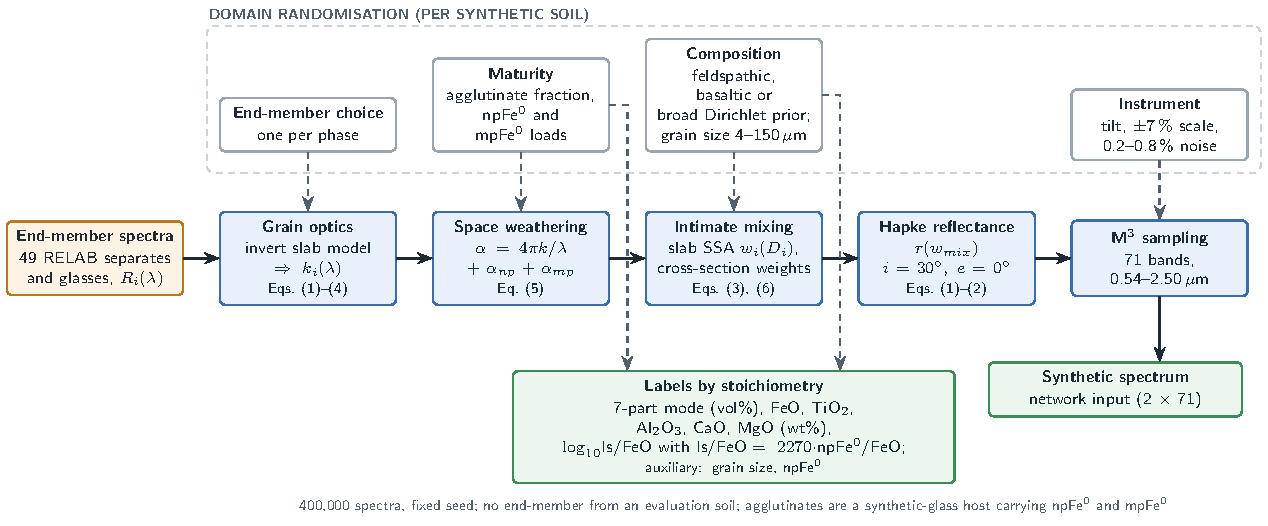
\includegraphics[width=\linewidth]{figures/fig_simulator}
\end{adjustwidth}
\caption{The domain-randomised physics simulator. Each end-member's imaginary index k($\lambda$) is obtained by inverting the equivalent-slab model; space weathering adds npFe$^{0}$ and mpFe$^{0}$ absorption; components mix in single-scattering albedo with cross-section weights and are converted to reflectance with the Hapke model; the spectrum is resampled to the 71 M$^{3}$ bands. Composition, grain size, maturity and instrument effects are randomised, and labels follow from stoichiometry.\label{fig2}}
\end{figure}

\subsubsection{Network}

The network (Figure 3, Table 1) reads two channels on the 71 bands, log reflectance and convex-hull continuum-removed reflectance, each standardised with statistics of the synthetic set only. Five one-dimensional convolutions, each followed by group normalisation (preferred to batch normalisation because fine-tuning batches are small) and GELU, with two max-pooling steps, feed a 256--128 trunk (0.36 M parameters). A Dirichlet head outputs concentrations $\boldsymbol\alpha = \mathrm{softplus}(\cdot)+0.05$ whose mean $\boldsymbol\alpha/\alpha_0$, with $\alpha_0=\sum_j\alpha_j$, is the seven-part composition; heteroscedastic Gaussian heads give a mean and log-variance for each oxide and log$_{10}$(Is/FeO); and auxiliary heads for grain size and npFe$^{0}$ are used during pretraining only.

\begin{figure}[H]
\begin{adjustwidth}{-\extralength}{0cm}
\centering
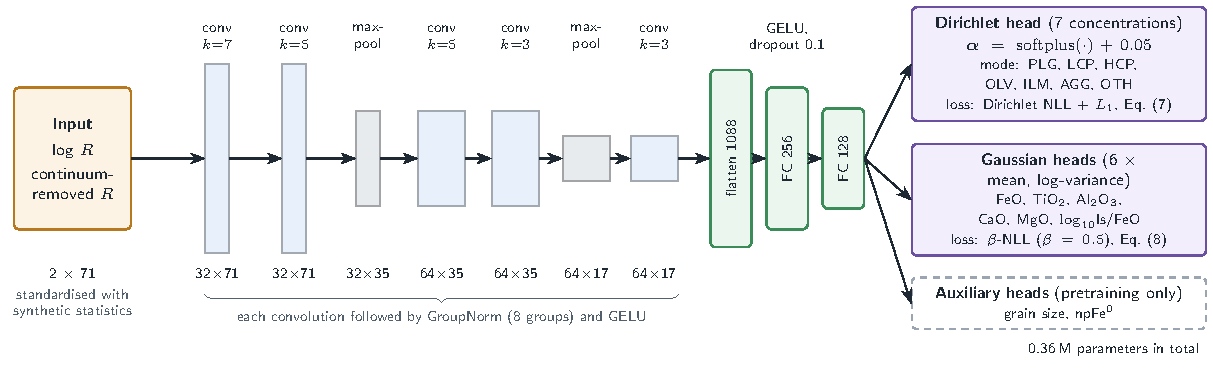
\includegraphics[width=\linewidth]{figures/fig_architecture}
\end{adjustwidth}
\caption{Network architecture. Tensor shapes are given as channels $\times$ bands. Each convolution is followed by group normalisation (8 groups) and GELU. The auxiliary heads are used during pretraining only.\label{fig3}}
\end{figure}

\subsubsection{Objective Functions}

The composition loss is the Dirichlet negative log-likelihood of the label-smoothed proportions, $\tilde{\mathbf y} = (\mathbf y+\epsilon)/(1+7\epsilon)$ with $\epsilon = 0.005$, plus an $L_1$ term on the mean:

\begin{equation}
\mathcal L_{comp} = -\frac{1}{7}\left[\ln\Gamma(\alpha_0) - \sum_j \ln\Gamma(\alpha_j) + \sum_j(\alpha_j-1)\ln\tilde y_j\right] + \lambda_1\,\frac{1}{7}\sum_j\left|\frac{\alpha_j}{\alpha_0} - y_j\right|
\label{eq7}
\end{equation}

with $\lambda_1 = 10$ fixed on synthetic data only. The scalar targets use the $\beta$-negative log-likelihood~\cite{seitzer2022} with $\beta=0.5$, which avoids the under-fitting of high-variance points caused by the plain Gaussian likelihood,

\begin{equation}
\mathcal L_{scal} = \frac{\sum_t m_t\,\mathrm{sg}\!\left[\sigma_t^{2\beta}\right]\tfrac12\left(\ln\sigma_t^2 + \frac{(y_t-\mu_t)^2}{\sigma_t^2}\right)}{\sum_t m_t}
\label{eq8}
\end{equation}

where $\mathrm{sg}$ stops the gradient and $m_t$ masks targets that are unavailable for a sample (modal mineralogy for the <45 $\upmu$m fraction; all targets except FeO for orbital spectra). The total loss is $\mathcal L_{comp} + \mathcal L_{scal}$, plus the auxiliary $\beta$-NLL terms during pretraining.

\subsubsection{Training}

Five ensemble members are pretrained on the synthetic set with different seeds (15 epochs, AdamW, one-cycle schedule, 20,000 spectra held out) and fine-tuned per cross-validation fold for 1500 steps (Table 1). In the full configuration (A4) each step combines 16 real training spectra, 16 synthetic replay spectra and 32 SSA-space mixup spectra, each a Dirichlet-weighted mixture of 2--3 training spectra combined with Equation (6) and labelled exactly (composition by volume, chemistry by mass, Is/FeO weighted by mass $\times$ FeO); real and mixed spectra receive the simulator's calibration and noise randomisation. The simpler configuration A2 uses the real spectra only. All hyperparameters were fixed from synthetic-only development runs and committed before any model was scored on real folds.

\subsubsection{Uncertainty and Identifiability}

The ensemble mean is the mean of the member means, and the ensemble variance is the mean of the member variances plus the variance of the member means~\cite{lakshminarayanan2017}. Because raw ensemble intervals are over-confident (Section 3.5), we calibrate them conformally~\cite{barber2021}: the normalised score $s_i = |y_i - \mu_i|/\sigma_i$ is computed from out-of-fold predictions of the other soils, and its $\lceil (1-a)(n+1)\rceil$-th smallest value $q_{1-a}$ gives the interval $\mu \pm q_{1-a}\,\sigma$. The exact CV+ variant uses models from which both the calibration soil and the test soil were held out (930 additional fine-tunes). For each target, the identifiability gate computes the skill

\begin{equation}
S = 1 - \frac{\mathrm{MAE}}{\mathrm{MAE}_{ref}}
\label{eq9}
\end{equation}

where $\mathrm{MAE}_{ref}$ is the error of the fraction-matched mean of the other soils, a zero-information reference, with a 95\% bootstrap interval over soils. A target is mapped only if the lower bound of that interval is above zero under leave-one-soil-out evaluation.

\subsubsection{Transfer to M$^{3}$}

Laboratory and M$^{3}$ reflectance differ in absolute scale. For zero-shot application, M$^{3}$ spectra are brought to the laboratory scale with the linear calibration of Korokhin et al.~\cite{korokhin2024},

\begin{equation}
A_{lab} = 1.685\,A_{M^3} + 0.0355
\label{eq10}
\end{equation}

and a site of Apollo mission X is predicted by the ensemble fine-tuned with all of mission X's soils held out (for the Luna and Chang'e sites, by the ensemble fine-tuned on all 19 soils). For orbital fine-tuning (LUMEN-M3-FT), the network is further trained for 600 steps (AdamW, learning rate 10$^{-4}$, weight decay 10$^{-4}$, cosine decay) on batches of 16 M$^{3}$ pixel spectra from the training sites, labelled with their site FeO and all other targets masked, and 16 laboratory spectra from that model's own training soils with all targets. The held-out site is predicted from its site spectrum.

\section{Results}

\subsection{Experimental Setup}

\subsubsection{Comparison Algorithms}

On the laboratory spectra every method uses identical spectra and folds. The classical baselines are the fraction-matched mean of the training soils (a zero-information reference); partial least squares (PLS), ridge regression and a random forest (RF) on LUMEN's 142 input values; and an RF on raw reflectance, all tuned by inner grouped cross-validation. The Fernández-Díaz et al. pipeline~\cite{fernandez2026} is re-implemented in full on the same spectra (db4 A2 + D2 wavelet coefficients; a 42 $\rightarrow$ 32 $\rightarrow$ 16 $\rightarrow$ 6 $\rightarrow$ 16 $\rightarrow$ 32 $\rightarrow$ 42 autoencoder trained on M$^{3}$ pixels as published or on our synthetic spectra; Lasso, linear SVR, RBF SVR and RF with the paper's search grids; and the no-autoencoder variant), giving twelve variants, of which "FD as published" is the M$^{3}$-trained autoencoder with RF. The outputs of Korokhin et al.~\cite{korokhin2024} and Jung et al.~\cite{jung2026} come from independent reproductions validated against the papers' printed numbers (46 of 65 and 32 of 34 gated targets), each scored as the paper scores itself.

On M$^{3}$ (Section 3.6) we compare zero-shot LUMEN, zero-shot LUMEN with a linear recalibration $y = a + b\hat y$ fitted on the training sites, LUMEN-M3-FT, and a ridge regression on the 128-dimensional trunk embedding ("LUMEN-embed + ridge") with the Fernández-Díaz variants retrained on M$^{3}$ site spectra, a linear model on two M$^{3}$ bands (R950/R750 and R750), the Lucey $\theta$ parameter~\cite{lucey2000} refitted on M$^{3}$, the published Lucey et al. constants and a refitted two-band model on the table's Clementine reflectances, and the training-fold mean.

\subsubsection{Parameter Settings}

Table 1 lists the fixed settings. All LUMEN hyperparameters were set from synthetic-only development runs and committed to version control with the evaluation protocol before any model was scored on real folds, and the later experiments (Sections 3.3, 3.6 and 3.7) were committed in the same way before they were run.

\begin{table}[H]
\caption{Fixed LUMEN settings.\label{tab1}}
\small
\begin{tabularx}{\textwidth}{LC}
\toprule
\textbf{Component} & \textbf{Setting} \\
\midrule
Simulator & 400,000 spectra; 49 end-members; grain size 4--150 $\upmu$m; scale $\pm$7\%; noise 0.2--0.8\% \\
Input & 2 $\times$ 71 (log R, continuum-removed R), standardised with synthetic statistics \\
Network & 5 conv layers (32/32/64/64/64; kernels 7/5/5/3/3), GroupNorm, GELU, 2 max-pools, trunk 256$\rightarrow$128; 0.36 M parameters \\
Losses & Dirichlet NLL + L1 ($\lambda_{1}$ = 10, $\epsilon$ = 0.005); $\beta$-NLL ($\beta$ = 0.5) \\
Pretraining & 5 members, 15 epochs, AdamW, one-cycle, batch 512 \\
Fine-tuning & 1500 steps, AdamW lr 3 $\times$ 10$^{-4}$, wd 10$^{-4}$, warm-up 100, cosine; batch 16 real + 32 SSA-mixup + 16 replay (A4) \\
Orbital fine-tuning & 600 steps, lr 10$^{-4}$, batch 16 M$^{3}$ + 16 lab spectra \\
Uncertainty & 5-member ensemble; normalised conformal (CV+) intervals; gate on bootstrap skill CI \\
Hardware & CPU only (4 cores); pretraining $\approx$ 45 min; one fine-tune $\approx$ 6 s \\
\bottomrule
\end{tabularx}
\end{table}

\subsubsection{Evaluation Protocols and Metrics}

Figure 4 summarises the evaluation design. Under leave-one-soil-out (LOSO, 19 folds), all four fractions of the held-out soil are excluded from fine-tuning, mixup and normalisation statistics. Leave-one-mission-out (LOMO, 6 folds: A11, A12, A14, A15, A16, A17) is the out-of-distribution test: holding out A16 removes every feldspathic soil, and holding out A17 every high-Ti soil. The primary metric is the per-soil mean absolute error (MAE): each soil's labelled fractions are averaged and then the 19 soils are averaged, so the number of independent units is the number of soils, not of spectra. R$^{2}$ and RMSE are reported per spectrum. Methods are compared with paired Wilcoxon signed-rank tests over soils~\cite{wilcoxon1945} with Holm correction~\cite{holm1979} over the 13 targets or over the comparators, and bootstrap confidence intervals are computed over soils.

\begin{figure}[H]
\begin{adjustwidth}{-\extralength}{0cm}
\centering
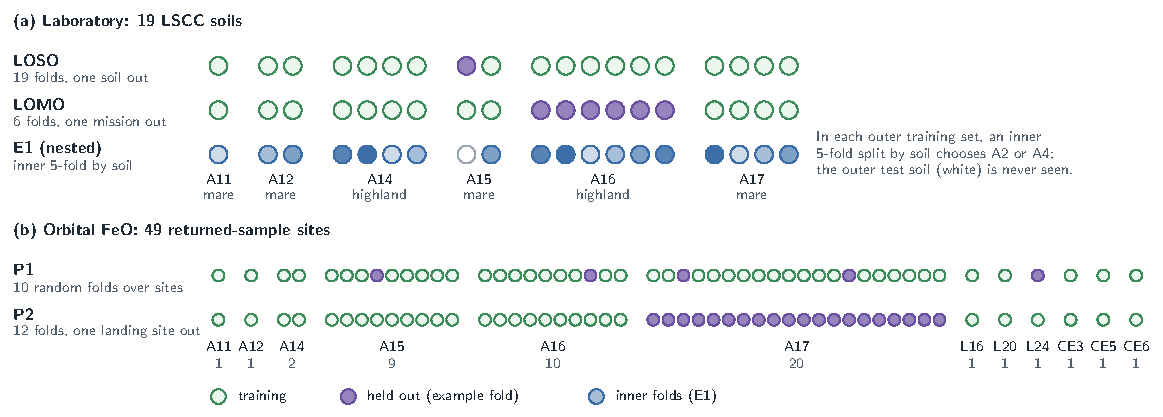
\includegraphics[width=\linewidth]{figures/fig_evaluation}
\end{adjustwidth}
\caption{Evaluation design. Laboratory models are evaluated by leave-one-soil-out and leave-one-mission-out cross-validation, with the A2/A4 configuration chosen by an inner grouped five-fold split of each outer training set. Orbital FeO is evaluated at the 49 returned-sample sites by ten-fold cross-validation over sites (P1, the protocol of~\cite{fernandez2026}) and by leave-one-landing-site-out (P2).\label{fig4}}
\end{figure}

\subsection{Simulator Validation}

Every self-test of the simulator passes. Each end-member's k($\lambda$) reproduces its measured reflectance to 7.8 $\times$ 10$^{-11}$. Truncating the composition prior lowers the 99th-percentile synthetic TiO$_{2}$ from 30.5 to 14.0 wt\% (LSCC maximum 10.7) and FeO from 31.8 to 24.4 wt\%. Modal composition multiplied by class-average phase chemistry reproduces the LSCC bulk oxides with r = 0.93--0.98, but mare TiO$_{2}$ is biased by +2.9 wt\%, which affects only the scale of the pretraining labels. The measured <45 $\upmu$m spectra are reproduced by mixing their sieve fractions to 0.6\% RMS. The median nearest-synthetic-neighbour distance of the 75 LSCC spectra is 0.102, against 0.144 between synthetic spectra, so the real data lie inside the synthetic distribution; yet a classifier separates real from synthetic spectra with an AUC of 0.97 (0.99 against noise-free synthetics), real soils being redder than their nearest synthetic neighbours. This sim-to-real gap is what fine-tuning must close.

\subsection{Accuracy on the LSCC Soils}

Table 2 gives per-soil MAEs. Under LOSO, LUMEN (A4) has a skill over the zero-information reference of 0.50 for composition and 0.72 for FeO. It has a lower error than each classical baseline on 12 of 13 targets, the exception always being olivine, and after Holm correction it is significantly better than PLS on 9 targets and than the mean of other soils on 10. Against the strongest baseline, a random forest on the same inputs, A4 is lower on 12 of 13 targets, but only maturity is significant after correction (for FeO, raw p = 0.005, Holm p = 0.064). Under LOMO every method degrades: A4's composition MAE rises from 2.66 to 4.70 vol\% and its FeO MAE from 1.26 to 2.59 wt\%. A4 remains lower than RF on 10 of 13 targets, significantly so for LCP, HCP and TiO$_{2}$, while for the "other" class no method beats the zero-information reference.

\begin{table}[H]
\caption{Per-soil MAE, LOSO / LOMO (composition in vol\%, oxides in wt\%, maturity in log$_{10}$ Is/FeO). Bold: lowest per row and protocol.\label{tab2}}
\begin{adjustwidth}{-\extralength}{0cm}
\small
\begin{tabularx}{\fulllength}{LCCCCC}
\toprule
\textbf{Target} & \textbf{Mean of others} & \textbf{PLS} & \textbf{Ridge} & \textbf{RF} & \textbf{LUMEN (A4)} \\
\midrule
PLG & 14.09 / 17.74 & 11.13 / 16.66 & 10.58 / 16.68 & 7.13 / 12.45 & \textbf{4.82 / 11.31} \\
LCP & 3.23 / 3.89 & 2.40 / 3.69 & 2.38 / 3.47 & 2.23 / 3.33 & \textbf{1.75 / 2.50} \\
HCP & 2.89 / 3.49 & 1.92 / 1.72 & 1.78 / 1.78 & 1.57 / 1.93 & \textbf{1.07 / 1.22} \\
OLV & 0.93 / 1.05 & 0.87 / 1.06 & 0.87 / 1.03 & \textbf{0.84 / 0.98} & 0.98 / 1.13 \\
ILM & 2.63 / 3.22 & 1.89 / 2.18 & 1.81 / 2.10 & 1.68 / 2.30 & \textbf{1.22 / 1.69} \\
AGG & 9.60 / 9.53 & 9.85 / 12.29 & 9.29 / 11.86 & 7.14 / 9.94 & \textbf{5.78 / 9.18} \\
OTH & 3.85 / \textbf{4.81} & 3.62 / 5.34 & 3.45 / 5.22 & 3.37 / 5.41 & \textbf{3.02} / 5.88 \\
FeO & 4.47 / 5.56 & 2.77 / 3.58 & 2.64 / 4.39 & 2.13 / 3.69 & \textbf{1.26 / 2.59} \\
TiO$_{2}$ & 2.67 / 3.28 & 1.70 / 2.30 & 1.63 / 1.90 & 1.43 / 2.27 & \textbf{0.70 / 1.37} \\
Al$_{2}$O$_{3}$ & 6.00 / 7.53 & 4.03 / 5.90 & 3.65 / 6.44 & 2.84 / 5.41 & \textbf{1.71 / 4.33} \\
CaO & 2.41 / 3.04 & 1.87 / 2.98 & 1.72 / 3.20 & 1.23 / 2.43 & \textbf{0.87 / 2.20} \\
MgO & 1.99 / 2.50 & 1.40 / 2.21 & 1.31 / 2.12 & 0.92 / \textbf{1.71} & \textbf{0.78} / 1.74 \\
log$_{10}$ Is/FeO & 0.31 / 0.30 & 0.20 / 0.24 & 0.22 / 0.21 & 0.20 / 0.23 & \textbf{0.11 / 0.15} \\
Composition (mean) & 5.32 / 6.25 & 4.53 / 6.13 & 4.31 / 6.02 & 3.42 / 5.19 & \textbf{2.66 / 4.70} \\
\bottomrule
\end{tabularx}
\end{adjustwidth}
\end{table}

Because the pre-registered primary model A4 is not the best configuration (Section 3.7), we repeated the choice between A4 and the simpler A2 inside each outer training fold by inner five-fold grouped cross-validation, keeping the outer estimate confirmatory. A2 was selected in every fold (19 of 19 under LOSO, 6 of 6 under LOMO). The selected model reaches 1.23 wt\% FeO, 0.55 wt\% TiO$_{2}$ and 2.35 vol\% composition under LOSO and, against RF, is lower on 12 of 13 targets (not olivine, 0.86 vs 0.84 vol\%) and significantly better after Holm correction on 8: PLG, LCP, HCP, ILM, FeO, TiO$_{2}$, Al$_{2}$O$_{3}$ and maturity (FeO 1.23 vs 2.13 wt\%, Holm p = 0.011). It is significant on 11 of 13 targets against PLS and ridge and on 10 against the mean of other soils. Under LOMO it is significantly better than RF on 6 targets (LCP, HCP, FeO, TiO$_{2}$, Al$_{2}$O$_{3}$ and maturity; FeO 2.63 wt\%). No A4--A2 difference is significant under either protocol. These runs use pretrained members regenerated on a different machine, which reproduce the stored per-soil MAEs to within 0.06 for every target, configuration and protocol. Figure 5 shows the LOSO predictions for four headline targets.

\begin{figure}[H]
\begin{adjustwidth}{-\extralength}{0cm}
\centering
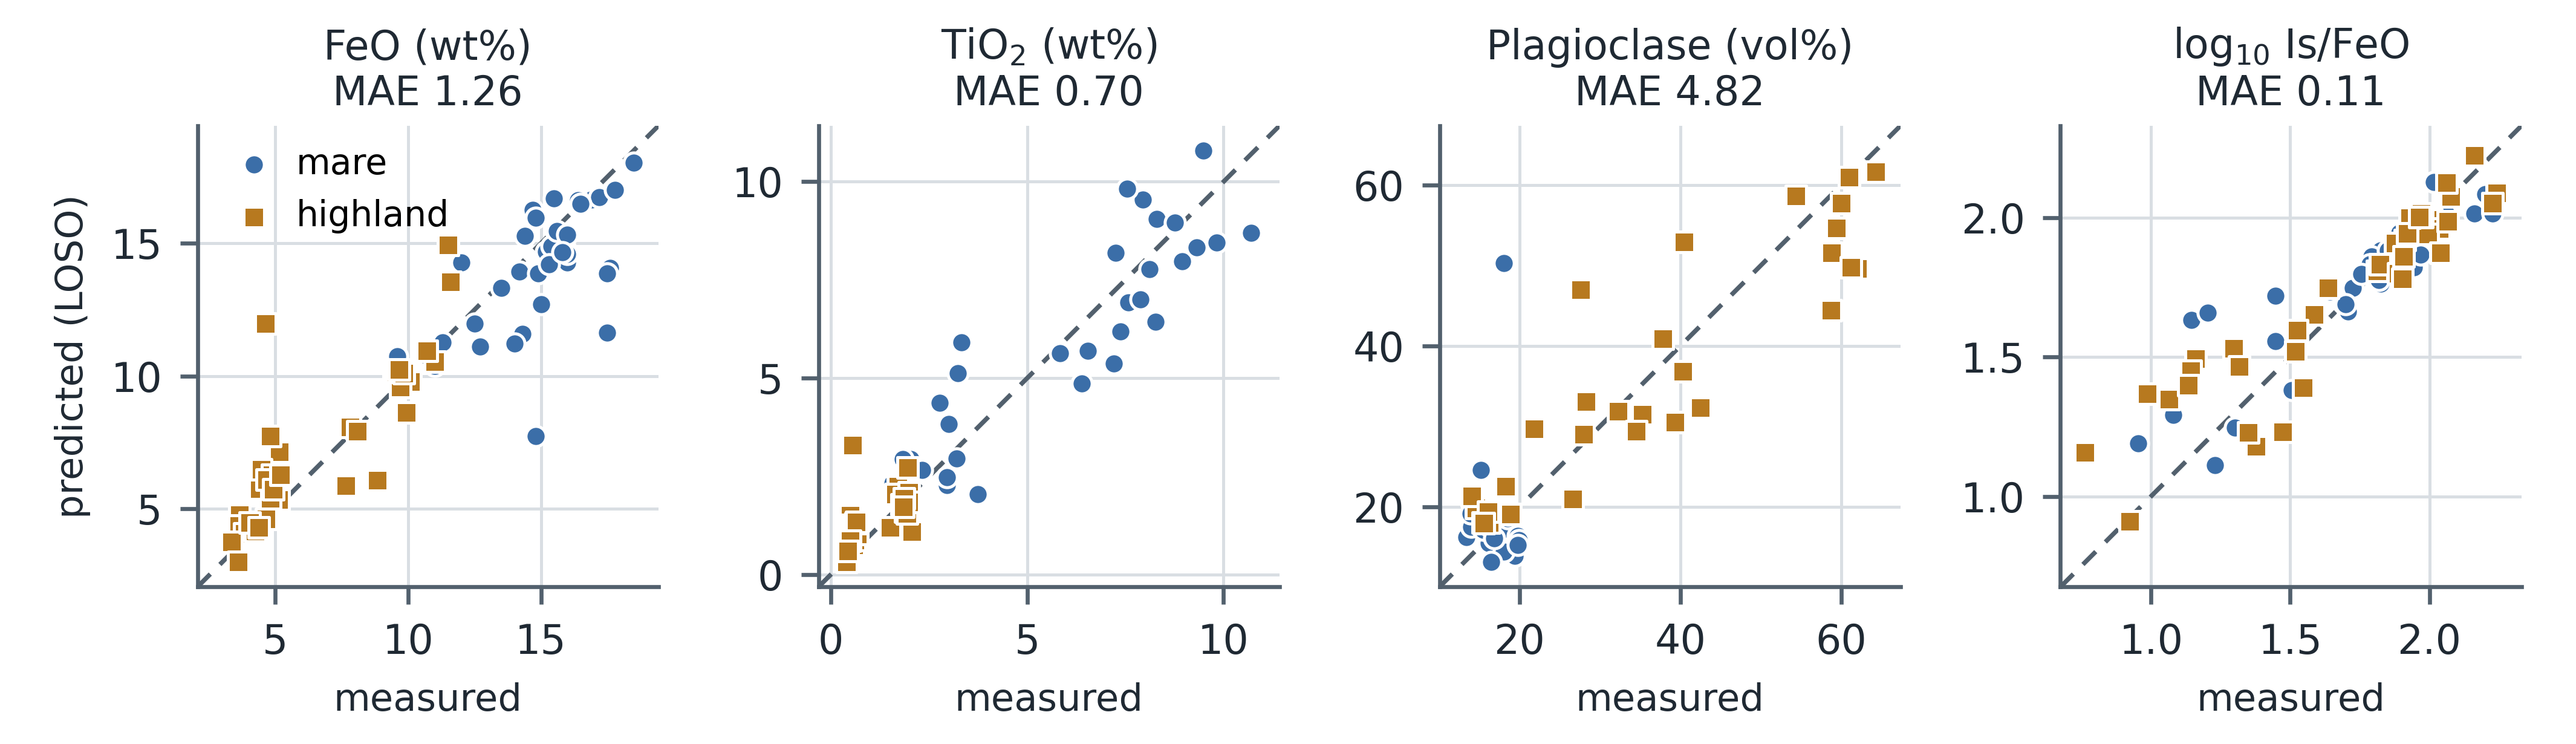
\includegraphics[width=\linewidth]{figures/fig05_pred_true}
\end{adjustwidth}
\caption{LUMEN (A4) predictions against measured values for the 19 LSCC soils under leave-one-soil-out, for FeO, TiO$_{2}$, plagioclase and maturity. Each point is one sieve fraction; the line is 1:1.\label{fig5}}
\end{figure}

\subsection{Comparison with Published Methods}

\subsubsection{Wavelet--Autoencoder FeO Regression~\cite{fernandez2026}}

This is the fairest comparison, because the pipeline is trained on exactly the same spectra and folds (Table 3, Figure 6). Under LOSO, LUMEN's FeO error (1.26 wt\%, R$^{2}$ = 0.85) is 42\% lower than that of FD as published (2.17 wt\%, R$^{2}$ = 0.62) and lower than all twelve variants, the best being wavelet $\rightarrow$ RBF SVR without the autoencoder (1.91 wt\%). Each paired test has p < 0.05, the test fixed in the protocol; with an additional Holm correction over the twelve variants, 3 of 12 remain significant (vs FD as published, Holm p = 0.069). Under LOMO, LUMEN has 2.59 wt\% against 3.48 for FD as published (p = 0.018) and 2.91 for the best variant (p = 0.49). Under LOSO the M$^{3}$-trained autoencoder is worse than the raw wavelet coefficients for 4 of 4 regressors, as in our reproduction of the original study (RF 1.55 vs 1.95 wt\% with the autoencoder), whereas under LOMO it helps the two linear regressors.

\begin{table}[H]
\caption{FeO (wt\%) on identical spectra and folds. "FD-AE-M3" is the published autoencoder, trained on M$^{3}$ pixels; "FD-AE-synth" is trained on our synthetic spectra; "FD-wavelet" has no autoencoder. The remaining FD variants are in the repository tables.\label{tab3}}
\begin{adjustwidth}{-\extralength}{0cm}
\small
\begin{tabularx}{\fulllength}{LCCCC}
\toprule
\textbf{Method} & \textbf{MAE LOSO} & \textbf{R$^{2}$ LOSO} & \textbf{MAE LOMO} & \textbf{R$^{2}$ LOMO} \\
\midrule
\textbf{LUMEN (A4)} & \textbf{1.26} & \textbf{0.85} & \textbf{2.59} & 0.57 \\
LUMEN (A2, pretrain + real) & 1.23 & 0.86 & 2.64 & 0.58 \\
FD-AE-M3 / RF (published) & 2.17 & 0.62 & 3.48 & 0.25 \\
FD-AE-M3 / Lasso & 2.48 & 0.55 & 3.09 & 0.39 \\
FD-AE-M3 / SVR-lin & 2.19 & 0.65 & 3.06 & 0.41 \\
FD-AE-M3 / SVR-RBF & 2.06 & 0.62 & 3.79 & 0.07 \\
FD-AE-synth / SVR-lin & 2.09 & 0.65 & 2.91 & 0.48 \\
FD-wavelet / SVR-RBF & 1.91 & 0.67 & 3.28 & 0.17 \\
FD-wavelet / Lasso & 2.07 & 0.70 & 3.95 & $-$0.01 \\
RF (LUMEN inputs) & 2.13 & 0.62 & 3.69 & 0.16 \\
RF (raw reflectance) & 2.19 & 0.58 & 3.45 & 0.27 \\
Mean of other soils & 4.47 & $-$0.06 & 5.56 & $-$0.70 \\
\bottomrule
\end{tabularx}
\end{adjustwidth}
\end{table}

\begin{figure}[H]
\begin{adjustwidth}{-\extralength}{0cm}
\centering
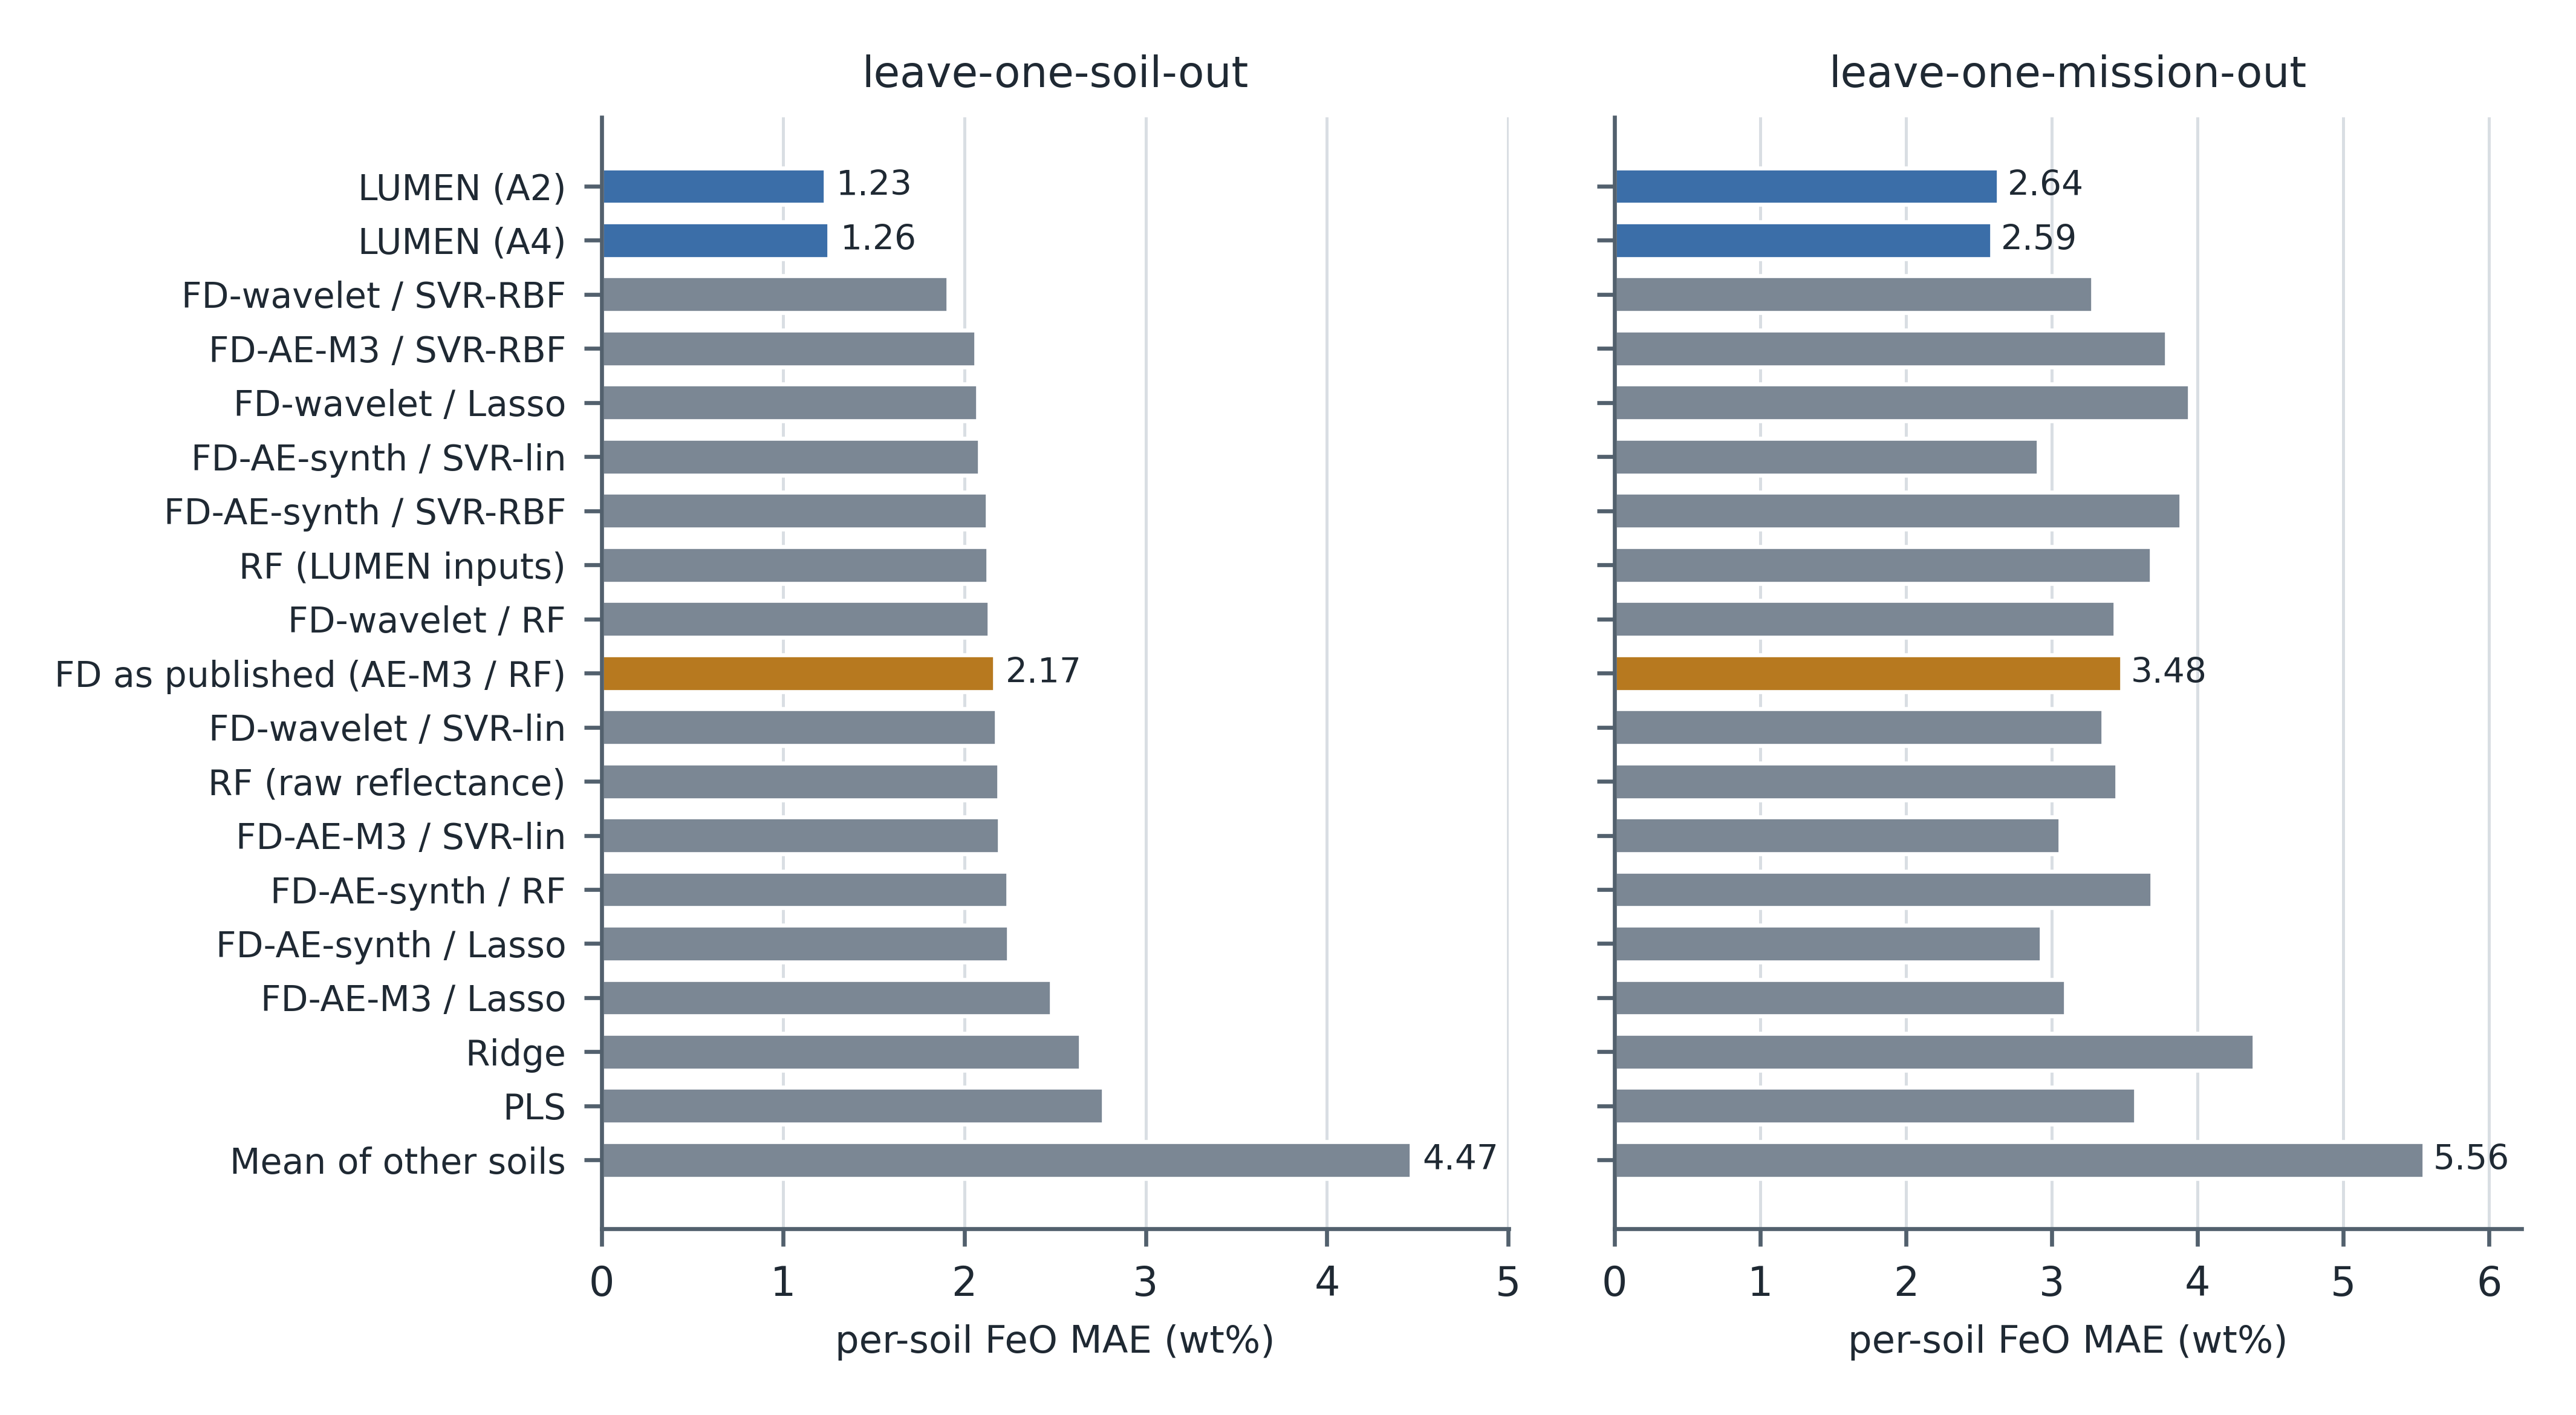
\includegraphics[width=\linewidth]{figures/fig06_fd_feo}
\end{adjustwidth}
\caption{Per-soil FeO error of LUMEN, the Fernández-Díaz et al. variants and the classical baselines on identical folds, under leave-one-soil-out (left) and leave-one-mission-out (right).\label{fig6}}
\end{figure}

\subsubsection{Shkuratov-Model Inversion~\cite{korokhin2024}}

Each method is scored on five-mineral proportions (CPX, OPX, OLV, PLG, ILM, renormalised to 100\%) over the three sieved fractions, as the reproduction of Korokhin et al. scores itself (Table 4). Under LOSO, LUMEN reduces the error for every mineral by 54--74\%, every difference being Holm-significant; for example, olivine is 1.91 against 7.44 points and plagioclase 5.55 against 12.08. Under LOMO, LUMEN is still lower on four of five minerals, significantly only for olivine, and slightly worse for plagioclase (12.64 vs 12.08). The inversion never sees an LSCC soil, whereas LUMEN is fine-tuned on the others, so the like-for-like comparison is LUMEN's zero-shot model (A0, physics-trained only): it is lower on three of five minerals, significantly only for olivine. LUMEN's Is/FeO also ranks the soils better than the inversion's nFe parameter, with Spearman $\rho$ of 0.72, 0.81 and 0.96 for the <10, 10--20 and 20--45 $\upmu$m fractions against 0.55, 0.37 and 0.44.

\begin{table}[H]
\caption{MAE of five-mineral proportions (percentage points), 19 soils.\label{tab4}}
\begin{adjustwidth}{-\extralength}{0cm}
\small
\begin{tabularx}{\fulllength}{LCCCCCC}
\toprule
\textbf{Mineral} & \textbf{Mean of others} & \textbf{Korokhin fit} & \textbf{LUMEN A0 (zero-shot)} & \textbf{LUMEN A4 (LOSO)} & \textbf{LUMEN A4 (LOMO)} & \textbf{Holm p, A4 vs fit (LOSO)} \\
\midrule
CPX & 6.78 & 5.30 & 8.18 & \textbf{2.24} & 3.14 & 0.007 \\
OPX & 9.18 & 8.37 & 8.98 & \textbf{3.25} & 6.86 & 0.007 \\
OLV & 2.21 & 7.44 & 2.58 & \textbf{1.91} & 2.50 & <0.001 \\
PLG & 18.44 & 12.08 & 10.40 & \textbf{5.55} & 12.64 & 0.007 \\
ILM & 6.26 & 5.24 & 3.06 & \textbf{2.39} & 4.06 & 0.007 \\
\bottomrule
\end{tabularx}
\end{adjustwidth}
\end{table}

\subsubsection{Hapke--Bayesian Inversion~\cite{jung2026}}

On the four test soils of Jung et al. (12001, 12030, 15071 and 71061, 20--45 $\upmu$m), scored on crystalline proportions, LUMEN's worst-case LOSO errors are 1.00 points for olivine, 1.24 for ilmenite and 7.95 for plagioclase, meeting all three published accuracy bounds (7, 10 and 30 points), whereas the converged inversion reaches 17.56 points for ilmenite. With four soils this is weak evidence: the zero-shot model also meets every bound, while the mean of other soils misses the ilmenite and plagioclase bounds. Across the four soils, LUMEN's Is/FeO correlates with the measured value at r = 0.99, against r $\approx$ 0.00 for the inversion's maturity index.

\subsection{Uncertainty and Identifiability}

Raw ensemble intervals are over-confident (Figure 7): for nominal 68/90/95\% intervals, mean empirical coverage is 0.59/0.82/0.89 under LOSO and 0.33/0.55/0.64 under LOMO. Normalised conformal calibration restores 0.68/0.90/0.95 under LOSO and 0.64/0.86/0.92 under LOMO. Exact CV+, which uses models that saw neither the calibration soil nor the test soil, gives 0.69/0.90/0.96 (LOSO) and 0.70/0.88/0.93 (LOMO), so the approximation is slightly conservative out of distribution. The identifiability gate passes 11 of 13 targets (Table 5). It withholds olivine, whose LOSO skill is $-$0.06 (CI $-$0.40 to 0.22), and the "other" class (0.22, CI $-$0.03 to 0.42); under LOMO the agglutinate fraction also loses significance (0.04, CI $-$0.34 to 0.25).

\begin{table}[H]
\caption{Skill over the zero-information reference with 95\% bootstrap CI.\label{tab5}}
\small
\begin{tabularx}{\textwidth}{LCCC}
\toprule
\textbf{Target} & \textbf{LOSO skill [CI]} & \textbf{LOMO skill [CI]} & \textbf{Mapped} \\
\midrule
PLG & 0.66 [0.47, 0.78] & 0.36 [0.19, 0.52] & yes \\
LCP & 0.46 [0.32, 0.59] & 0.36 [0.20, 0.50] & yes \\
HCP & 0.63 [0.53, 0.71] & 0.65 [0.55, 0.74] & yes \\
OLV & $-$0.06 [$-$0.40, 0.22] & $-$0.08 [$-$0.38, 0.16] & \textbf{no} \\
ILM & 0.54 [0.40, 0.64] & 0.47 [0.36, 0.57] & yes \\
AGG & 0.40 [0.16, 0.54] & 0.04 [$-$0.34, 0.25] & yes \\
OTH & 0.22 [$-$0.03, 0.42] & $-$0.22 [$-$0.51, $-$0.03] & \textbf{no} \\
FeO & 0.72 [0.61, 0.80] & 0.53 [0.44, 0.60] & yes \\
TiO$_{2}$ & 0.74 [0.61, 0.82] & 0.58 [0.45, 0.65] & yes \\
Al$_{2}$O$_{3}$ & 0.71 [0.56, 0.82] & 0.43 [0.28, 0.54] & yes \\
CaO & 0.64 [0.50, 0.75] & 0.28 [0.16, 0.38] & yes \\
MgO & 0.61 [0.37, 0.77] & 0.31 [0.05, 0.47] & yes \\
log$_{10}$ Is/FeO & 0.63 [0.56, 0.71] & 0.50 [0.32, 0.61] & yes \\
\bottomrule
\end{tabularx}
\end{table}

\begin{figure}[H]
\begin{adjustwidth}{-\extralength}{0cm}
\centering
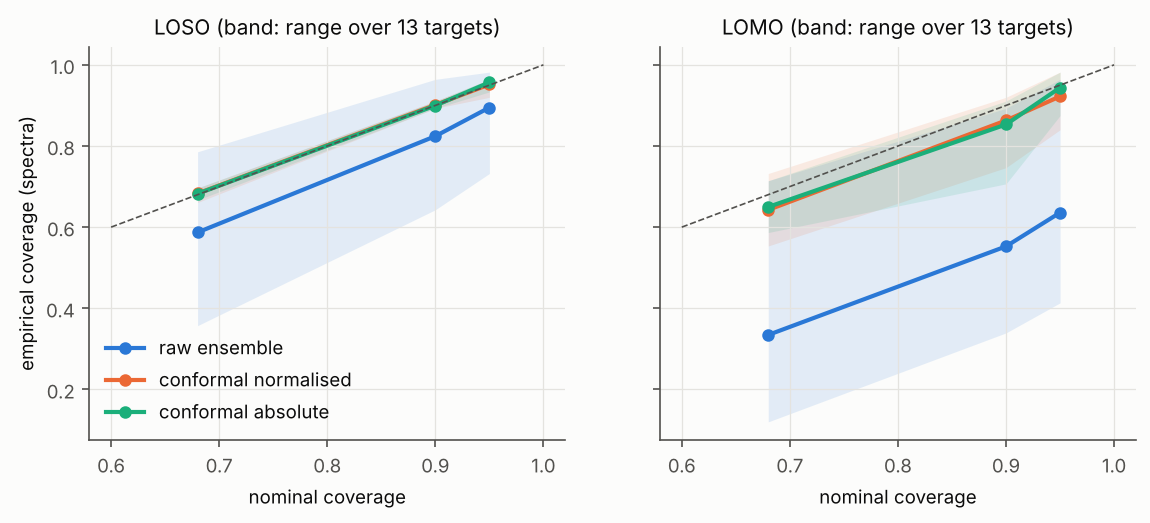
\includegraphics[width=\linewidth]{figures/step05_coverage}
\end{adjustwidth}
\caption{Empirical against nominal interval coverage for the raw ensemble and after conformal calibration, under leave-one-soil-out and leave-one-mission-out.\label{fig7}}
\end{figure}

\subsection{FeO from M$^{3}$ Spectra at Returned-Sample Sites}

This experiment tests the base method on its own task, orbital FeO, against the ground truth it was calibrated on~\cite{fernandez2026,qiu2025}, under two protocols (Figure 4): P1, the base study's own 10-fold cross-validation over sites, comparable with its published MAE of 2.29 wt\%; and P2, leave-one-landing-site-out, in which all stations of a mission are held out together because they share terrain and are spatially autocorrelated. All 49 sites have M$^{3}$ coverage and are scored (Table 6, Figure 8).

\begin{table}[H]
\caption{FeO (wt\%) at the 49 returned-sample sites, P1 (10-fold, seed 42) / P2 (leave-one-landing-site-out), 3 $\times$ 3-pixel site spectra. Bias is predicted minus laboratory FeO. Every method except the zero-shot model and the Lucey et al. constants is fitted inside each training fold.\label{tab6}}
\begin{adjustwidth}{-\extralength}{0cm}
\small
\begin{tabularx}{\fulllength}{LCCCCCCCC}
\toprule
\textbf{Method} & \textbf{P1 MAE} & \textbf{P1 RMSE} & \textbf{P1 R$^{2}$} & \textbf{P1 bias} & \textbf{P2 MAE} & \textbf{P2 RMSE} & \textbf{P2 R$^{2}$} & \textbf{P2 bias} \\
\midrule
LUMEN-M3 (zero-shot) & 6.81 & 7.52 & $-$1.30 & $-$5.29 & 6.81 & 7.52 & $-$1.30 & $-$5.29 \\
LUMEN-M3 + recalibration & 4.39 & 5.17 & $-$0.09 & $-$0.04 & 5.11 & 6.34 & $-$0.63 & 0.17 \\
\textbf{LUMEN-M3-FT} & 2.20 & 3.01 & 0.63 & $-$1.19 & 3.27 & 4.02 & 0.34 & $-$1.01 \\
LUMEN-embed + ridge & 2.01 & 2.56 & 0.73 & $-$0.60 & 2.60 & 3.16 & 0.59 & $-$0.38 \\
FD-AE-M3 / RF (published) & 1.90 & 2.71 & 0.70 & 0.01 & 3.58 & 4.21 & 0.28 & 1.29 \\
FD-AE-M3 / Lasso & 2.11 & 2.71 & 0.70 & 0.01 & 3.07 & 3.78 & 0.42 & 0.78 \\
FD-AE-M3 / SVR-lin & 2.30 & 2.95 & 0.65 & $-$0.37 & 2.27 & 2.86 & 0.67 & $-$0.44 \\
FD-AE-M3 / SVR-RBF & 2.12 & 2.85 & 0.67 & $-$0.02 & 3.27 & 3.86 & 0.40 & 0.56 \\
FD-wavelet / RF & 1.96 & 2.72 & 0.70 & $-$0.32 & 3.21 & 3.88 & 0.39 & 0.72 \\
FD-wavelet / Lasso & 2.19 & 2.81 & 0.68 & $-$0.24 & 2.44 & 3.49 & 0.50 & 0.20 \\
FD-wavelet / SVR-lin & 2.49 & 3.16 & 0.59 & $-$0.61 & 2.54 & 3.41 & 0.53 & $-$0.02 \\
FD-wavelet / SVR-RBF & 2.40 & 3.39 & 0.53 & $-$0.03 & 4.39 & 5.94 & $-$0.44 & 1.31 \\
Two M$^{3}$ bands (R950/R750, R750) & 1.99 & 2.43 & 0.76 & 0.00 & 2.11 & 2.54 & 0.74 & $-$0.16 \\
Lucey $\theta$ (M$^{3}$, refitted) & 3.26 & 3.70 & 0.44 & 0.00 & 4.30 & 5.04 & $-$0.03 & $-$0.03 \\
Lucey et al. constants (Clementine) $^{a}$ & 1.25 & 1.72 & 0.88 & $-$0.17 & 1.25 & 1.72 & 0.88 & $-$0.17 \\
Two Clementine bands (refitted) & 1.34 & 1.74 & 0.88 & 0.03 & 1.82 & 2.32 & 0.78 & $-$0.31 \\
Training-fold mean & 4.34 & 5.07 & $-$0.04 & 0.00 & 4.78 & 5.69 & $-$0.32 & 0.03 \\
\bottomrule
\end{tabularx}
\end{adjustwidth}
\noindent{\footnotesize{$^{a}$ In-sample. The published constants~\cite{lucey2000} were derived from returned-sample sites, and nothing is fitted here, so this row is not a held-out estimate and is not comparable with the others.}}
\end{table}

In the primary test (P2), LUMEN-M3-FT has a lower MAE than FD as published (3.27 vs 3.58 wt\%) but is the more accurate of the two at only 24 of the 49 sites, and the difference is not significant (Wilcoxon p = 0.74; Holm p = 1.00 over 13 comparators). It is significantly better only than the training-fold mean (Holm p < 0.001) and significantly worse than the two M$^{3}$ bands (Holm p = 0.009), FD-AE-M3 / SVR-lin (Holm p = 0.029), the two Clementine bands (Holm p = 0.001) and the in-sample Lucey et al. constants (Holm p < 0.001). Under P1, FD as published (1.90 wt\%) is close to our reproduction of the original study (1.95 wt\%) and below its published 2.29 wt\%~\cite{fernandez2026}; LUMEN-M3-FT (2.20 wt\%) differs significantly from no FD variant and not from the two M$^{3}$ bands, is significantly less accurate than the two Clementine bands (Holm p = 0.020) and significantly more accurate than the refitted Lucey $\theta$ on M$^{3}$ (Holm p = 0.020).

The result is robust. Over six P1 seeds LUMEN-M3-FT averages 2.13 wt\% (2.08--2.20) and FD as published 1.91 wt\% (1.81--1.97), FD being lower under every seed, and with each strip's centre pixel instead of the 3 $\times$ 3 block LUMEN-M3-FT has 3.26 wt\% against 3.35 wt\% (Holm p = 1.00) and remains significantly worse than the two M$^{3}$ bands (2.02 wt\%, Holm p = 0.006). Under P2, conformal intervals for LUMEN-M3-FT cover 0.63, 0.92 and 0.98 of the sites at nominal 68, 90 and 95\% (raw ensemble 0.51, 0.76 and 0.86), with mean half-widths of 4.6 wt\% at 68\% and 10.6 wt\% at 95\%.

\begin{figure}[H]
\begin{adjustwidth}{-\extralength}{0cm}
\centering
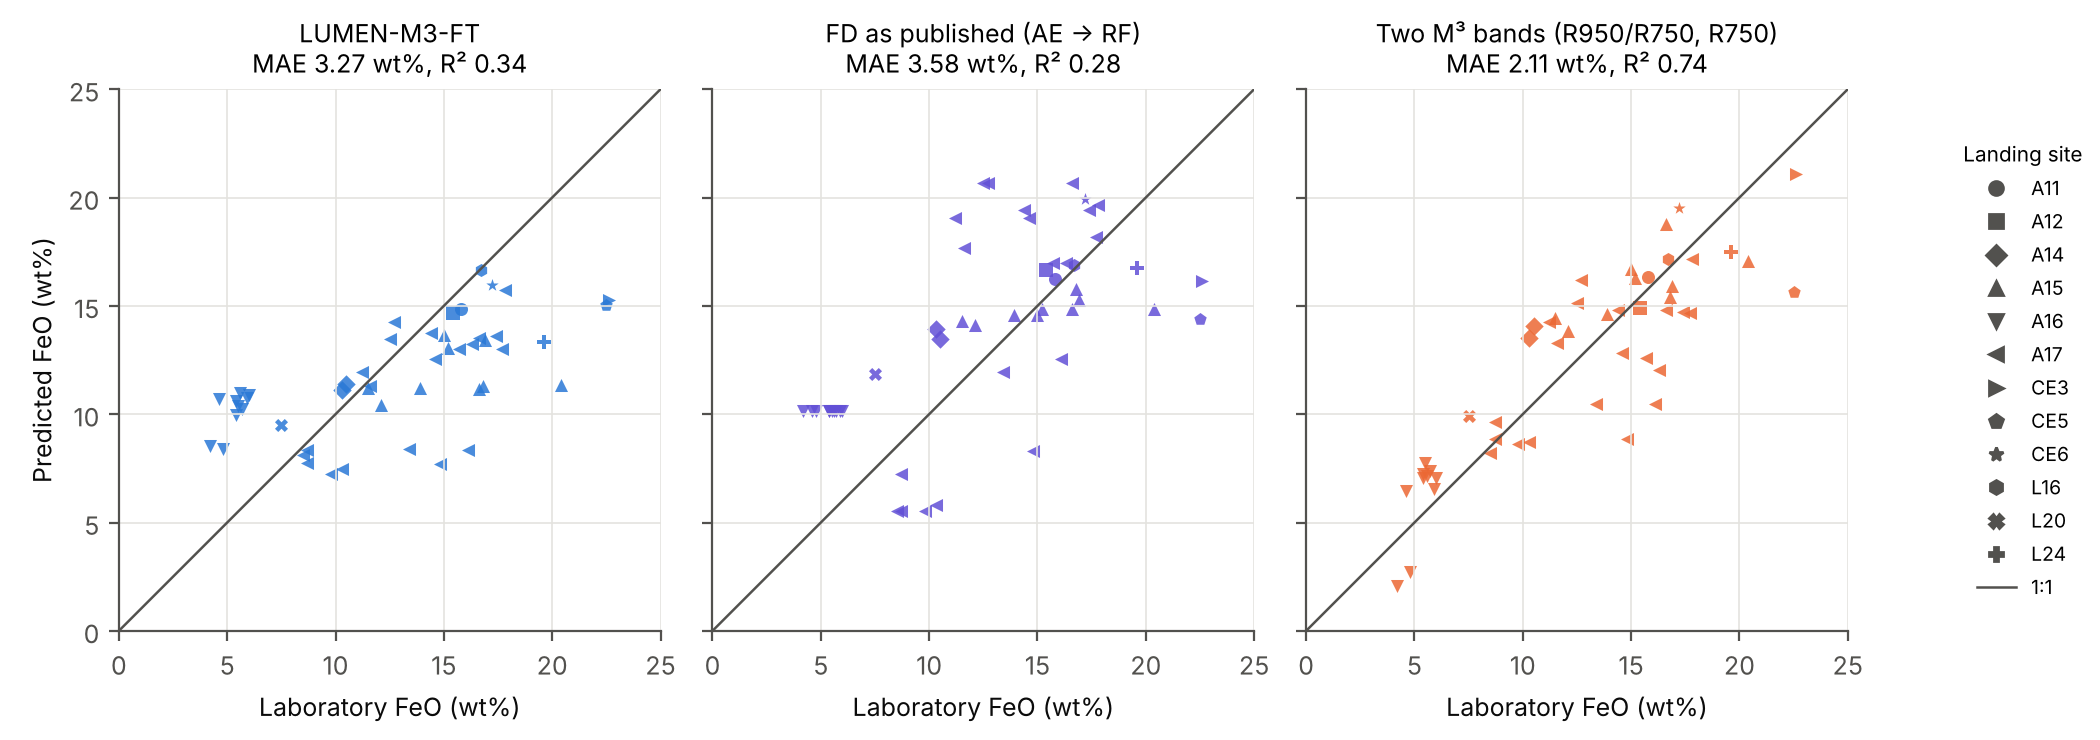
\includegraphics[width=\linewidth]{figures/fig05_m3_sites}
\end{adjustwidth}
\caption{Predicted against laboratory FeO at the 49 returned-sample sites under P2 (leave-one-landing-site-out), for LUMEN-M3-FT, FD as published and the two-M$^{3}$-band linear model. Marker shape gives the landing site; the line is 1:1.\label{fig8}}
\end{figure}

\subsection{Ablations and Parameter Analysis}

Pretraining helps, but the pre-registered primary model is not the best configuration (Table 7). The pretrained A2 has a lower error than the same network trained from scratch (A1) on all 13 targets under LOSO, although, the targets being correlated, no single difference is significant after Holm correction; under LOMO two are (HCP and maturity). SSA-mixup and synthetic replay lower the error of the pretrained network (A4 vs A2) on only 1 of 13 targets, with no significant difference, and help a network trained from scratch under LOSO (12 of 13 targets) but not under LOMO (2 of 13). The zero-shot A0, the physics-only analogue of a simulator-trained inversion, has a composition MAE of 9.1 vol\%, far above every fine-tuned variant.

\begin{table}[H]
\caption{Ablations: per-soil MAE, LOSO / LOMO. A4 is the pre-registered primary model.\label{tab7}}
\begin{adjustwidth}{-\extralength}{0cm}
\small
\begin{tabularx}{\fulllength}{LCCCCCC}
\toprule
\textbf{Target} & \textbf{A0 zero-shot} & \textbf{A1 scratch, real} & \textbf{A1m scratch + mixup} & \textbf{A2 pretrain + real} & \textbf{A3 pretrain + mixup} & \textbf{A4 full} \\
\midrule
PLG & 13.99 / 13.99 & 4.84 / 11.76 & 4.21 / 12.01 & 4.17 / 12.01 & 4.25 / 12.31 & 4.82 / 11.31 \\
LCP & 4.88 / 4.88 & 1.58 / 2.45 & 1.57 / 2.57 & 1.42 / 2.12 & 1.41 / 2.15 & 1.75 / 2.50 \\
HCP & 4.51 / 4.51 & 1.21 / 1.72 & 1.19 / 1.82 & 0.85 / 1.09 & 0.94 / 1.15 & 1.07 / 1.22 \\
OLV & 1.22 / 1.22 & 0.91 / 1.02 & 0.92 / 1.04 & 0.86 / 1.03 & 0.93 / 1.06 & 0.98 / 1.13 \\
ILM & 1.83 / 1.83 & 1.30 / 1.95 & 1.30 / 2.07 & 1.08 / 1.70 & 1.22 / 1.90 & 1.22 / 1.69 \\
AGG & 25.53 / 25.53 & 6.19 / 9.61 & 5.68 / 9.34 & 5.42 / 9.64 & 5.50 / 9.45 & 5.78 / 9.18 \\
OTH & 12.00 / 12.00 & 2.78 / 5.63 & 2.70 / 5.82 & 2.69 / 5.82 & 2.77 / 6.06 & 3.02 / 5.88 \\
FeO & 4.57 / 4.57 & 1.46 / 2.75 & 1.32 / 3.00 & 1.23 / 2.64 & 1.23 / 2.71 & 1.26 / 2.59 \\
TiO$_{2}$ & 3.91 / 3.91 & 0.82 / 1.43 & 0.76 / 1.57 & 0.56 / 1.08 & 0.66 / 1.36 & 0.70 / 1.37 \\
Al$_{2}$O$_{3}$ & 3.79 / 3.79 & 1.74 / 4.35 & 1.58 / 4.62 & 1.51 / 4.24 & 1.61 / 4.54 & 1.71 / 4.33 \\
CaO & 1.69 / 1.69 & 0.76 / 2.12 & 0.74 / 2.29 & 0.73 / 2.20 & 0.76 / 2.29 & 0.87 / 2.20 \\
MgO & 1.84 / 1.84 & 0.82 / 1.58 & 0.69 / 1.69 & 0.71 / 1.74 & 0.71 / 1.75 & 0.78 / 1.74 \\
log$_{10}$ Is/FeO & 0.30 / 0.30 & 0.15 / 0.19 & 0.14 / 0.18 & 0.12 / 0.14 & 0.13 / 0.15 & 0.11 / 0.15 \\
Composition (mean) & 9.14 / 9.14 & 2.69 / 4.88 & 2.51 / 4.95 & 2.36 / 4.77 & 2.43 / 4.87 & 2.66 / 4.70 \\
\bottomrule
\end{tabularx}
\end{adjustwidth}
\end{table}

Without the physics, the network already improves on classical regression: A1 is significantly better than RF on 5 of 13 targets under LOSO (PLG, ILM, FeO, TiO$_{2}$ and Al$_{2}$O$_{3}$) and 3 under LOMO, and the pretrained A2 on 8 and 6 targets, which is why its choice is moved inside the cross-validation (Section 3.3).

Four design alternatives were pretrained and fine-tuned with the A4 recipe and two members each, against members 0--1 of the main network (Table 8; FeO 1.32 wt\% under LOSO and 2.62 wt\% under LOMO). Log reflectance alone performs on par (no significant difference), so the continuum-removed channel adds nothing measurable, whereas the continuum-removed channel alone is significantly worse on 6 targets under LOSO and 8 under LOMO (FeO 2.09 and 3.86 wt\%). The MLP is significantly worse for LCP under LOSO but significantly better on 4 targets under LOMO (PLG, FeO, Al$_{2}$O$_{3}$ and CaO; FeO 2.30 wt\%), and the 1-D ResNet shows no significant difference.

\begin{table}[H]
\caption{Design alternatives against the main network (2 members each, 13 targets, Holm correction over targets). "Lower MAE": number of targets on which the variant's per-soil MAE is below the main network's. "Better / worse": number of targets with a Holm-significant difference in the variant's favour or against it.\label{tab8}}
\begin{adjustwidth}{-\extralength}{0cm}
\small
\begin{tabularx}{\fulllength}{LCCCCC}
\toprule
\textbf{Variant} & \textbf{Parameters} & \textbf{LOSO: lower MAE} & \textbf{LOSO: better / worse} & \textbf{LOMO: lower MAE} & \textbf{LOMO: better / worse} \\
\midrule
Main network (log R + continuum-removed, CNN) & 0.36 M & --- & --- & --- & --- \\
Log R only & 0.36 M & 10 / 13 & 0 / 0 & 5 / 13 & 0 / 0 \\
Continuum-removed only & 0.36 M & 0 / 13 & 0 / 6 & 1 / 13 & 0 / 8 \\
MLP & 0.07 M & 0 / 13 & 0 / 1 & 9 / 13 & 4 / 0 \\
1-D ResNet & 0.42 M & 7 / 13 & 0 / 0 & 8 / 13 & 0 / 0 \\
\bottomrule
\end{tabularx}
\end{adjustwidth}
\end{table}

\subsection{Application to M$^{3}$ Scenes}

On the Apollo 16 landing-site pixel the published calibration (Equation (10)) reproduces the LSCC 62231 spectrum to 9.1\% RMS, and a line re-derived from that pixel to 1.4\%; LUMEN estimates 5.0 wt\% FeO there (62231: 4.9 wt\%; Apollo 16 mean: 4.6 wt\%) and over-estimates TiO$_{2}$ (2.1 vs 0.6 wt\%), a sanity check only, since 62231 is in the final training set. In the Shapley scene (Figure 9) the 11 identifiable targets show the expected contrasts (FeO 10.2 wt\% on mare and 6.6 wt\% on highland; Al$_{2}$O$_{3}$ 20.0 and 24.3 wt\%) and fresh craters stand out as immature. The published high-Ca pyroxene map of the same strip~\cite{korokhin2024} is anti-correlated with LUMEN's (r = $-$0.79), placing more clinopyroxene in the highlands than in the mare, and its maturity parameter is nearly unrelated to LUMEN's Is/FeO (r = $-$0.28). Destriping lowers stripe amplitude by 26--47\% and leaves the maps correlated at r = 0.90--0.99 with the undestriped ones. At Aristarchus, LUMEN finds much less olivine and more plagioclase in the crystalline fraction than the posterior abundances of Jung et al.~\cite{jung2026} (52\% vs 29\% plagioclase in region B); since LUMEN's olivine output fails the identifiability gate, this is a domain-shift warning, not evidence against that study.

\begin{figure}[H]
\begin{adjustwidth}{-\extralength}{0cm}
\centering
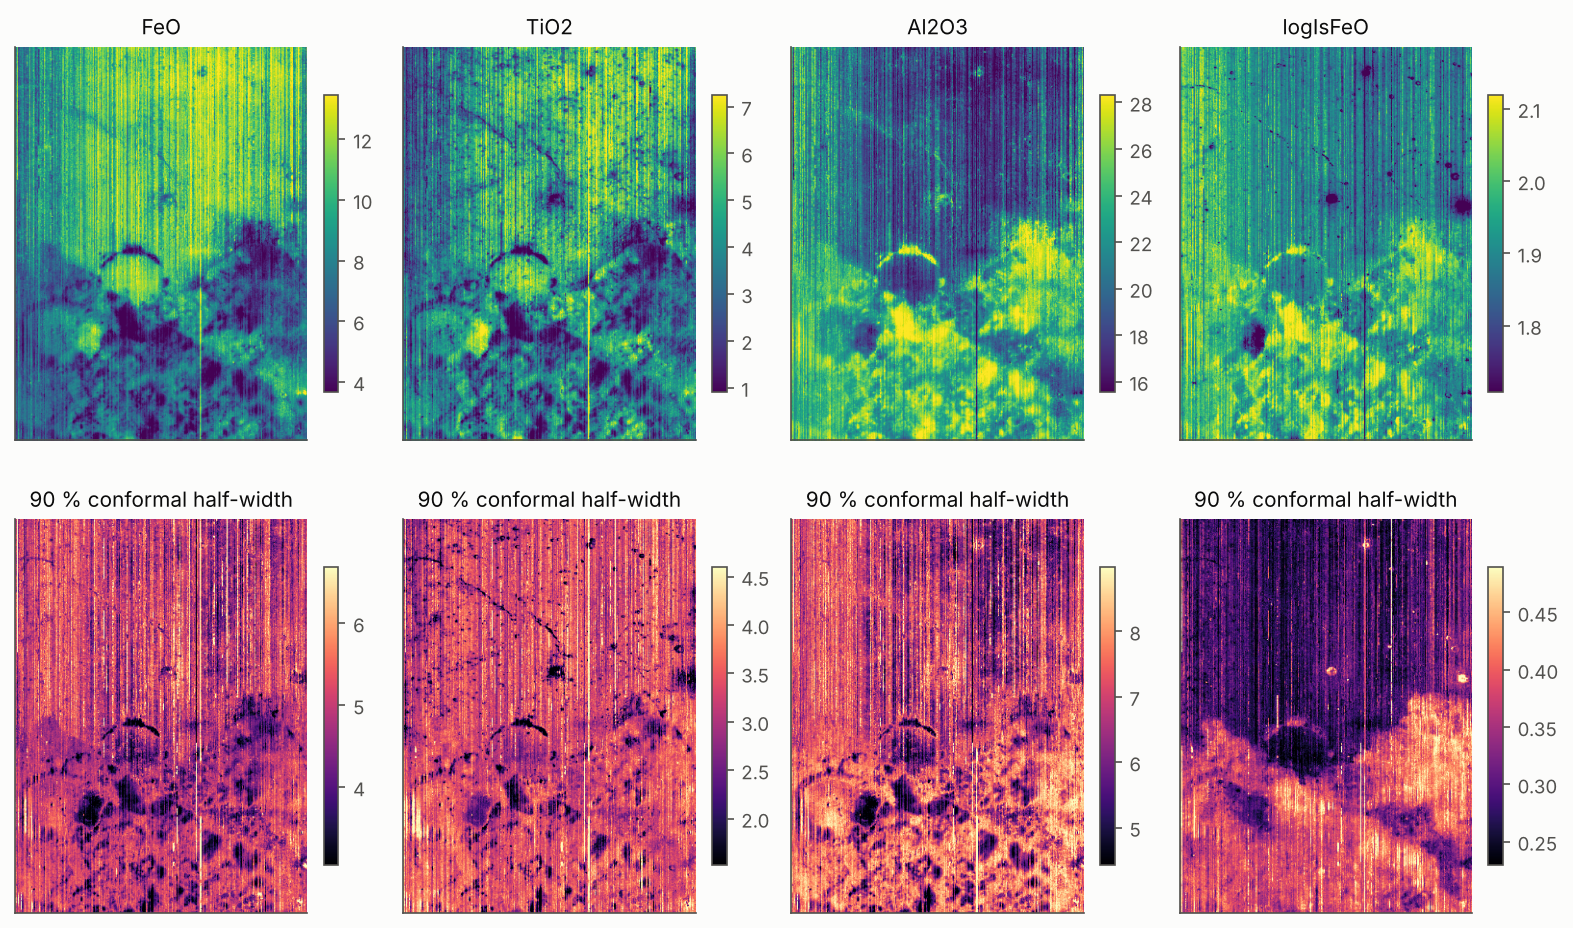
\includegraphics[width=\linewidth]{figures/step07_shapley_maps}
\end{adjustwidth}
\caption{LUMEN maps of the Shapley-region M$^{3}$ strip for identifiable targets, with conformal interval half-widths. Olivine and "other" are withheld by the identifiability gate.\label{fig9}}
\end{figure}

\section{Discussion}

\subsection{What Carries the Gain on Laboratory Spectra}

The decisive step is calibration against real soils. The zero-shot network is the weakest LUMEN variant and, for composition, worse than the zero-information reference, whereas any fine-tuning on returned soils cuts the error by a factor of two to four. Together with the simulator analysis, in which the LSCC spectra lie inside the synthetic distribution yet remain separable from it, this shows that a physics model good enough to cover the data is not, by itself, good enough to be inverted.

The other ingredients contribute differently. Learning on the whole spectrum is a real part of the gain, since the network trained from scratch already beats a tuned random forest, but the convolutional design is a reasonable rather than an optimal choice: the continuum-removed channel adds nothing measurable, a 1-D ResNet performs alike, and an MLP generalises better to an unseen mission on four targets. Physics pretraining helps consistently but is significant only out of distribution, so we regard the simulator as a source of a better starting representation rather than a calibrated forward model. SSA-space mixup and replay added nothing once the network was pretrained, either because pretraining already supplies the smoothness over composition space that mixup was meant to add, or because the cross-section mixing weights cannot be validated: sieve-fraction spectra mix linearly to 0.6\% RMS, but the LSCC chemistry does not constrain the mass proportions well enough. Finally, choosing the configuration inside each training fold keeps the significant advantage over the random forest, which therefore does not depend on picking the configuration after seeing the results.

\subsection{Comparison with Published Methods}

The three comparisons are not equally informative. Only the Fernández-Díaz et al.~\cite{fernandez2026} pipeline was trained on exactly the same spectra and folds, so LUMEN's 42\% lower FeO error is the fair comparison; it also confirms that the autoencoder stage removes information. Korokhin et al.~\cite{korokhin2024} and Jung et al.~\cite{jung2026} never see an LSCC soil, so LUMEN's margins over them mostly measure the value of calibrating against returned soils: like for like, the zero-shot model beats the Shkuratov inversion significantly only for olivine, and Jung et al.'s four test soils are too few for strong conclusions. A practically relevant difference is maturity, which both physics methods rank worse than LUMEN's calibrated Is/FeO.

\subsection{Laboratory-to-Orbit Transfer}

On the base method's own task the result goes against LUMEN. Holding out whole landing sites (P2) raises the error of almost every fitted method relative to random folds (P1), but by very different amounts: the random-forest and RBF-SVR models lose most, 55--88\% (FD as published rises from 1.90 to 3.58 wt\%), LUMEN-M3-FT 49\%, and the two-M$^{3}$-band regression and linear SVRs least (6\% and $-$1 to +2\%). Under random folds, flexible models can learn the spectral signature of a landing site from its neighbouring stations, so random-fold errors at these sites, including FD's published 2.29 wt\%, overstate the accuracy expected at a new location.

LUMEN-M3-FT's predictions are compressed toward the mean (Figure 8), over-estimating the Apollo 16 highland sites by 4.8 wt\% on average and under-estimating the FeO-rich Chang'e-3, Chang'e-5 and Luna 24 sites by 6.3--7.5 wt\%. With a few dozen training sites per fold, a linear model on two band parameters makes better use of the orbital labels, and even a ridge regression on LUMEN's embedding (2.60 wt\%, not tested for significance) does better than fine-tuning the whole network. The laboratory-to-orbit gap is large: zero-shot predictions are worse than the training-fold mean, linear recalibration removes their bias but not their error, and orbital fine-tuning halves the error without closing the gap. The calibration itself is uncertain, since the published transfer reproduces the Apollo 16 laboratory spectrum to 9.1\% RMS against 1.4\% for a line re-derived from that pixel.

The in-sample Lucey/Clementine result does not show that the Lucey algorithm beats the other methods at a new site, because its constants were derived from returned-sample sites; it does show that a single parameter, $\theta$, carries most of the FeO signal there. Refitted inside each fold, the two-band model is also more accurate on the table's Clementine reflectances than on our M$^{3}$ site spectra (1.82 vs 2.11 wt\% under P2), so part of the orbital error may lie in the M$^{3}$ site spectra themselves (calibration, photometry, site localisation) rather than in the regressors. In the mapped scenes, the largest disagreements with published maps occur exactly where LUMEN's gate withholds the output (olivine) or where the published network itself recovers poorly (pyroxene split, maturity).

\subsection{Uncertainty and Identifiability}

Deep ensembles alone are over-confident, more so out of distribution, and normalised conformal calibration restores near-nominal coverage at no extra training cost, also on orbit, where at 95\% the intervals average $\pm$10.6 wt\% and are therefore honest rather than useful. The gate makes explicit a limitation that other methods leave implicit: olivine abundance in these soils cannot be predicted better than by the mean of the other soils, by any method we tested, so olivine and "other" maps from physics inversions reflect their priors and end-member sets unless independently supported. Because the soils contain little olivine ($\leq$5 vol\%), this is a statement about the LSCC domain, not a claim that olivine is undetectable where it is abundant.

\subsection{Limitations}

The ground truth is small (19 laboratory soils, 56 spectra with modal mineralogy, and 49 orbital sites, 20 of them Apollo 17 stations), and several numerically large differences do not survive correction. Laboratory spectra of sieved fractions under fixed geometry differ from M$^{3}$ pixels that integrate rock, regolith and topography over about 140 m, and the orbital comparison relies on site coordinates and a single linear calibration. The simulator's chemistry labels are biased for mare TiO$_{2}$ (+2.9 wt\%) and its maturity scale rests on one constant, which limits the zero-shot model. The physics baselines enter through independent reproductions, and the Fernández-Díaz pipeline was re-implemented from its description. The orbital fine-tuning recipe was fixed in advance and not tuned; searching it, or smaller networks, needs more orbital ground truth. Transfer to other sensors, such as Chandrayaan-2 IIRS, is not tested here.

\section{Conclusions}

LUMEN, a physics-pretrained and sample-calibrated network, retrieves lunar soil mineralogy, chemistry and maturity from M$^{3}$-band reflectance with calibrated intervals and an explicit statement of which outputs are identifiable. On identical laboratory spectra and folds, under a protocol fixed before scoring, it reduces FeO error by 42\% relative to a published wavelet--autoencoder pipeline and mineral-proportion errors by 54--74\% relative to a Shkuratov-model inversion, meets the published accuracy bounds of a Hapke--Bayesian inversion, and, with its configuration chosen inside the cross-validation, is significantly more accurate than a tuned random forest on 8 of 13 targets. Most of the improvement over physics-only methods comes from calibrating against returned soils; learning on the whole spectrum and physics pretraining add to it, the convolutional design is not uniquely good, and the proposed SSA-space augmentation does not help.

On M$^{3}$ spectra at 49 returned-sample sites, LUMEN does not transfer zero-shot, and after orbital fine-tuning it is not significantly better than the published pipeline and significantly worse than a two-band linear regression, so for orbital FeO at these sites the deep model offers no advantage over simple band regressions. Olivine and minor glass abundances are not identifiable from these spectra by any method we tested. Future work should enlarge the orbital ground truth, which is now the limiting resource, add independent map-level checks against Kaguya and Clementine FeO products, and extend the approach to IIRS with an explicit sensor model.


\vspace{6pt}

\authorcontributions{}
\funding{}
\dataavailability{All code, the version-controlled evaluation protocol, every intermediate table and the staged input data, with their SHA-256 manifests, are available at \url{https://github.com/DSheth2004/lumen-lunar-dl}. RELAB spectra are available from the PDS Geosciences Node spectral library, and M$^{3}$ data from the NASA Planetary Data System. The returned-sample FeO table is Supplementary Table 1 of Qiu et al.~\cite{qiu2025}.}
\acknowledgments{We thank the RELAB facility at Brown University and the Lunar Soil Characterization Consortium for the laboratory data, and the M$^{3}$ team and the Planetary Data System for the orbital data.}
\conflictsofinterest{}

\abbreviations{Abbreviations}{
The following abbreviations are used in this manuscript:
\\

\noindent
\begin{tabular}{@{}ll}
AGG & agglutinitic glass\\
CV+ & cross-validation-plus conformal prediction\\
FD & Fernández-Díaz et al. pipeline\\
HCP / LCP & high- / low-Ca pyroxene\\
ILM & ilmenite\\
LOSO / LOMO & leave-one-soil-out / leave-one-mission-out\\
LSCC & Lunar Soil Characterization Consortium\\
M$^{3}$ & Moon Mineralogy Mapper\\
MAE & mean absolute error\\
npFe$^{0}$ / mpFe$^{0}$ & nanophase / microphase metallic iron\\
OLV & olivine\\
OTH & other phases\\
PLG & plagioclase\\
RELAB & Reflectance Experiment Laboratory\\
RF & random forest\\
SSA & single-scattering albedo\\
\end{tabular}
}

\begin{adjustwidth}{-\extralength}{0cm}
\reftitle{References}
\begin{thebibliography}{999}
\bibitem[pieters2009]{pieters2009}
Pieters, C.M.; Boardman, J.; Buratti, B.; Chatterjee, A.; Clark, R.; Glavich, T.; Green, R.; Head, J., III; Isaacson, P.; Malaret, E.; et al. The Moon Mineralogy Mapper (M3) on Chandrayaan-1. \emph{Curr. Sci.} {\bf 2009}, \emph{96}, 500--505.
\bibitem[green2011]{green2011}
Green, R.O.; Pieters, C.; Mouroulis, P.; Eastwood, M.; Boardman, J.; Glavich, T.; Isaacson, P.; Annadurai, M.; Besse, S.; Barr, D.; et al. The Moon Mineralogy Mapper (M3) imaging spectrometer for lunar science: Instrument description, calibration, on-orbit measurements, science data calibration and on-orbit validation. \emph{J. Geophys. Res.} {\bf 2011}, \emph{116}, E00G19. \url{https://doi.org/10.1029/2011je003797}.
\bibitem[lucey2000]{lucey2000}
Lucey, P.G.; Blewett, D.T.; Jolliff, B.L. Lunar iron and titanium abundance algorithms based on final processing of Clementine ultraviolet-visible images. \emph{J. Geophys. Res. Planets} {\bf 2000}, \emph{105}, 20297--20305. \url{https://doi.org/10.1029/1999je001117}.
\bibitem[bhatt2012]{bhatt2012}
Bhatt, M.; Mall, U.; Bugiolacchi, R.; McKenna-Lawlor, S.; Banaszkiewicz, M.; Nathues, A.; Ullaland, K. Lunar iron abundance determination using the 2-$\upmu$m absorption band parameters. \emph{Icarus} {\bf 2012}, \emph{220}, 51--64. \url{https://doi.org/10.1016/j.icarus.2012.04.010}.
\bibitem[bhatt2015]{bhatt2015}
Bhatt, M.; Mall, U.; Wöhler, C.; Grumpe, A.; Bugiolacchi, R. A comparative study of iron abundance estimation methods: Application to the western nearside of the Moon. \emph{Icarus} {\bf 2015}, \emph{248}, 72--88. \url{https://doi.org/10.1016/j.icarus.2014.10.023}.
\bibitem[sun2016]{sun2016}
Sun, L.; Ling, Z.; Zhang, J.; Li, B.; Chen, J.; Wu, Z.; Liu, J. Lunar iron and optical maturity mapping: Results from partial least squares modeling of Chang'E-1 IIM data. \emph{Icarus} {\bf 2016}, \emph{280}, 183--198. \url{https://doi.org/10.1016/j.icarus.2016.07.010}.
\bibitem[xia2019]{xia2019}
Xia, W.; Wang, X.; Zhao, S.; Jin, H.; Chen, X.; Yang, M.; Wu, X.; Hu, C.; Zhang, Y.; Shi, Y.; et al. New maps of lunar surface chemistry. \emph{Icarus} {\bf 2019}, \emph{321}, 200--215. \url{https://doi.org/10.1016/j.icarus.2018.10.031}.
\bibitem[wang2021]{wang2021}
Wang, X.; Zhang, J.; Ren, H. Lunar surface chemistry observed by the KAGUYA multiband imager. \emph{Planet. Space Sci.} {\bf 2021}, \emph{209}, 105360. \url{https://doi.org/10.1016/j.pss.2021.105360}.
\bibitem[qiu2022]{qiu2022}
Qiu, D.; Li, F.; Yan, J.; Gao, W.; Chong, Z. Machine learning for inversing FeO and TiO2 content on the Moon: Method and comparison. \emph{Icarus} {\bf 2022}, \emph{373}, 114778. \url{https://doi.org/10.1016/j.icarus.2021.114778}.
\bibitem[yang2023]{yang2023}
Yang, C.; Zhang, X.; Bruzzone, L.; Liu, B.; Liu, D.; Ren, X.; Benediktsson, J.A.; Liang, Y.; Yang, B.; Yin, M.; et al. Comprehensive mapping of lunar surface chemistry by adding Chang'e-5 samples with deep learning. \emph{Nat. Commun.} {\bf 2023}, \emph{14}, 7554. \url{https://doi.org/10.1038/s41467-023-43358-0}.
\bibitem[zhang2023]{zhang2023}
Zhang, L.; Zhang, X.; Yang, M.; Xiao, X.; Qiu, D.; Yan, J.; Xiao, L.; Huang, J. New maps of major oxides and Mg\# of the lunar surface from additional geochemical data of Chang'E-5 samples and KAGUYA multiband imager data. \emph{Icarus} {\bf 2023}, \emph{397}, 115505. \url{https://doi.org/10.1016/j.icarus.2023.115505}.
\bibitem[shi2026]{shi2026}
Shi, X.; Chen, J.; Wang, J.; Liu, S.; Tong, X.; Li, J.; Yan, Z.; Wen, S.; Xie, H.; He, Z.; et al. Refined lunar global chemistry mapping using farside ground truth information gathered by Chang'e-6. \emph{Nat. Sens.} {\bf 2026}, \emph{1}, 232--240. \url{https://doi.org/10.1038/s44460-025-00021-z}.
\bibitem[ma2022]{ma2022}
Ma, M.; Li, B.; Chen, S.; Lu, T.; Lu, P.; Lu, Y.; Jin, Q. Global estimates of lunar surface chemistry derived from LRO diviner data. \emph{Icarus} {\bf 2022}, \emph{371}, 114697. \url{https://doi.org/10.1016/j.icarus.2021.114697}.
\bibitem[wu2024]{wu2024}
Wu, S.; Chen, J.; Xue, C.; Pan, Y.; Zhang, C. Global Inversion of Lunar Surface Oxides by Adding Chang'e-5 Samples. \emph{Remote Sens.} {\bf 2024}, \emph{16}, 1812. \url{https://doi.org/10.3390/rs16101812}.
\bibitem[fernandez2025]{fernandez2025}
Fernández-Díaz, J.; de Cos Juez, F.J.; Sánchez Lasheras, F.; Gracia Rodriguez, J. Spectral Parameter-Based Prediction of Lunar FeO Content Using Random Forest Regression. \emph{Mathematics} {\bf 2025}, \emph{13}, 2802. \url{https://doi.org/10.3390/math13172802}.
\bibitem[fernandez2026]{fernandez2026}
Fernández-Díaz, J.; Sánchez Lasheras, F.; Rodríguez, J.G.; Álvarez, S.I.; Marqués Sierra, A.L.; de Cos Juez, F.J. Global Lunar FeO Mapping via Wavelet--Autoencoder Feature Learning from M3 Hyperspectral Data. \emph{Mathematics} {\bf 2026}, \emph{14}, 254. \url{https://doi.org/10.3390/math14020254}.
\bibitem[hapke1993]{hapke1993}
Hapke, B. \emph{Theory of Reflectance and Emittance Spectroscopy}; Cambridge University Press: Cambridge, UK, 1993.
\bibitem[hapke2001]{hapke2001}
Hapke, B. Space weathering from Mercury to the asteroid belt. \emph{J. Geophys. Res. Planets} {\bf 2001}, \emph{106}, 10039--10073. \url{https://doi.org/10.1029/2000je001338}.
\bibitem[lucey2011]{lucey2011}
Lucey, P.G.; Riner, M.A. The optical effects of small iron particles that darken but do not redden: Evidence of intense space weathering on Mercury. \emph{Icarus} {\bf 2011}, \emph{212}, 451--462. \url{https://doi.org/10.1016/j.icarus.2011.01.022}.
\bibitem[pieters2016]{pieters2016}
Pieters, C.M.; Noble, S.K. Space weathering on airless bodies. \emph{J. Geophys. Res. Planets} {\bf 2016}, \emph{121}, 1865--1884. \url{https://doi.org/10.1002/2016je005128}.
\bibitem[lili2011]{lili2011}
Li, S.; Li, L. Radiative transfer modeling for quantifying lunar surface minerals, particle size, and submicroscopic metallic Fe. \emph{J. Geophys. Res. Planets} {\bf 2011}, \emph{116}, 2011JE003837. \url{https://doi.org/10.1029/2011je003837}.
\bibitem[sunlucey2021]{sunlucey2021}
Sun, L.; Lucey, P.G. Unmixing Mineral Abundance and Mg\# With Radiative Transfer Theory: Modeling and Applications. \emph{J. Geophys. Res. Planets} {\bf 2021}, \emph{126}, e2020JE006691. \url{https://doi.org/10.1029/2020je006691}.
\bibitem[trang2019]{trang2019}
Trang, D.; Lucey, P.G. Improved space weathering maps of the lunar surface through radiative transfer modeling of Kaguya multiband imager data. \emph{Icarus} {\bf 2019}, \emph{321}, 307--323. \url{https://doi.org/10.1016/j.icarus.2018.11.014}.
\bibitem[shkuratov1999]{shkuratov1999}
Shkuratov, Y.; Starukhina, L.; Hoffmann, H.; Arnold, G. A Model of Spectral Albedo of Particulate Surfaces: Implications for Optical Properties of the Moon. \emph{Icarus} {\bf 1999}, \emph{137}, 235--246. \url{https://doi.org/10.1006/icar.1998.6035}.
\bibitem[korokhin2024]{korokhin2024}
Korokhin, V.; Surkov, Y.; Mall, U.; Kaydash, V.; Velichko, S.; Velikodsky, Y.; Shalygina, O. Applying machine learning to a nonlinear spectral mixing model for mapping lunar soils composition using CHANDRAYAAN-1 M3 data. \emph{Planet. Space Sci.} {\bf 2024}, \emph{244}, 105870. \url{https://doi.org/10.1016/j.pss.2024.105870}.
\bibitem[jung2026]{jung2026}
Jung, J.I.; Lapôtre, M.G.A.; Milliken, R.E.; Minson, S.E. Remote Compositional Analyses of Space-weathered Lunar Maria. \emph{Planet. Sci. J.} {\bf 2026}, \emph{7}, 18. \url{https://doi.org/10.3847/psj/ae2b57}.
\bibitem[lin2026]{lin2026}
Lin, Q.; Liu, C.; Han, D.; Liu, W.; Bo, Z.; Zhang, P. A Hapke Physics-Guided Deep Autoencoder for Lunar Hyperspectral Unmixing. \emph{Remote Sens.} {\bf 2026}, \emph{18}, 1123. \url{https://doi.org/10.3390/rs18081123}.
\bibitem[li2012]{li2012}
Li, S.; Li, L.; Milliken, R.; Song, K. Hybridization of partial least squares and neural network models for quantifying lunar surface minerals. \emph{Icarus} {\bf 2012}, \emph{221}, 208--225. \url{https://doi.org/10.1016/j.icarus.2012.07.023}.
\bibitem[grumpe2018]{grumpe2018}
Grumpe, A.; Mengewein, N.; Rommel, D.; Mall, U.; Wöhler, C. Interpreting spectral unmixing coefficients: From spectral weights to mass fractions. \emph{Icarus} {\bf 2018}, \emph{299}, 1--14. \url{https://doi.org/10.1016/j.icarus.2017.07.008}.
\bibitem[surkov2025]{surkov2025}
Surkov, Y.; Mall, U.; Korokhin, V. High resolution olivine abundance mapping in the Copernicus crater combining spectral data of Chandrayaan-1 M3 and Kaguya MI. \emph{Planet. Space Sci.} {\bf 2025}, \emph{256}, 106039. \url{https://doi.org/10.1016/j.pss.2025.106039}.
\bibitem[qiu2025]{qiu2025}
Qiu, D.; Yan, J.; Liu, B. Global chemical composition maps of oxide distributions on the Lunar surface. \emph{Commun. Earth Environ.} {\bf 2025}, \emph{6}, 940. \url{https://doi.org/10.1038/s43247-025-02914-w}.
\bibitem[taylor2001]{taylor2001}
Taylor, L.A.; Pieters, C.M.; Keller, L.P.; Morris, R.V.; McKay, D.S. Lunar Mare Soils: Space weathering and the major effects of surface-correlated nanophase Fe. \emph{J. Geophys. Res. Planets} {\bf 2001}, \emph{106}, 27985--27999. \url{https://doi.org/10.1029/2000je001402}.
\bibitem[taylor2010]{taylor2010}
Taylor, L.A.; Pieters, C.; Patchen, A.; Taylor, D.S.; Morris, R.V.; Keller, L.P.; McKay, D.S. Mineralogical and chemical characterization of lunar highland soils: Insights into the space weathering of soils on airless bodies. \emph{J. Geophys. Res. Planets} {\bf 2010}, \emph{115}, 2009JE003427. \url{https://doi.org/10.1029/2009je003427}.
\bibitem[relab2004]{relab2004}
Pieters, C.M.; Hiroi, T. RELAB (Reflectance Experiment Laboratory): A NASA Multiuser Spectroscopy Facility. In Proceedings of the 35th Lunar and Planetary Science Conference, League City, TX, USA, 15--19 March 2004; Abstract 1720.
\bibitem[qiu2025jgr]{qiu2025jgr}
Qiu, D.; Chen, W.; Yan, J.; Yi, S. FeO and TiO2 Maps of the Lunar Polar Regions Derived From the Clementine Data. \emph{J. Geophys. Res. Planets} {\bf 2025}, \emph{130}, e2024JE008753. \url{https://doi.org/10.1029/2024JE008753}.
\bibitem[seitzer2022]{seitzer2022}
Seitzer, M.; Tavakoli, A.; Antic, D.; Martius, G. On the Pitfalls of Heteroscedastic Uncertainty Estimation with Probabilistic Neural Networks. In Proceedings of the International Conference on Learning Representations (ICLR), Virtual, 25--29 April 2022.
\bibitem[lakshminarayanan2017]{lakshminarayanan2017}
Lakshminarayanan, B.; Pritzel, A.; Blundell, C. Simple and Scalable Predictive Uncertainty Estimation Using Deep Ensembles. In \emph{Advances in Neural Information Processing Systems 30}; Curran Associates: Red Hook, NY, USA, 2017; pp. 6402--6413.
\bibitem[barber2021]{barber2021}
Barber, R.F.; Candès, E.J.; Ramdas, A.; Tibshirani, R.J. Predictive inference with the jackknife+. \emph{Ann. Stat.} {\bf 2021}, \emph{49}, 486--507. \url{https://doi.org/10.1214/20-aos1965}.
\bibitem[wilcoxon1945]{wilcoxon1945}
Wilcoxon, F. Individual Comparisons by Ranking Methods. \emph{Biom. Bull.} {\bf 1945}, \emph{1}, 80--83. \url{https://doi.org/10.2307/3001968}.
\bibitem[holm1979]{holm1979}
Holm, S. A Simple Sequentially Rejective Multiple Test Procedure. \emph{Scand. J. Stat.} {\bf 1979}, \emph{6}, 65--70.
\end{thebibliography}
\end{adjustwidth}
\end{document}
